\documentclass[runningheads]{llncs}

\usepackage[T1]{fontenc}
\usepackage{graphicx}
\usepackage{placeins}
\usepackage{xcolor}
\usepackage{booktabs}
\usepackage{colortbl}
% Light rule between table rows, for readability.
% Institutional-function colors (figs/PALETTE.md): information layer and consequence layer, as in Fig. 2.
\definecolor{fninfo}{HTML}{5B6B7D}
\definecolor{keyline}{HTML}{B3BEC9}
\definecolor{keybg}{HTML}{FBFAF7}
\definecolor{fncons}{HTML}{9C4A78}
\newcommand{\fnmark}[1]{\textcolor{#1}{\rule{0.62em}{0.62em}}\nobreak\hspace{0.35em}}
% Let floats share pages with text instead of taking near-empty float pages.
\renewcommand{\topfraction}{0.92}
\renewcommand{\bottomfraction}{0.5}
\renewcommand{\textfraction}{0.06}
\renewcommand{\floatpagefraction}{0.85}
\renewcommand{\dbltopfraction}{0.92}
\renewcommand{\dblfloatpagefraction}{0.85}
\setcounter{topnumber}{4}
\setcounter{totalnumber}{5}
\newcommand{\rowline}{\arrayrulecolor{black!22}\specialrule{0.4pt}{2pt}{2pt}\arrayrulecolor{black}}
\usepackage{array}
\usepackage{multirow}
\usepackage[inline]{enumitem}
\usepackage{xurl}
\usepackage{microtype}
\usepackage{amssymb}
\usepackage{natbib}
\setcitestyle{numbers,square,comma}
\usepackage{hyperref}
\usepackage[capitalize,noabbrev]{cleveref}
\usepackage{soul}

\begin{document}
\raggedbottom % short pages end with space at the bottom, not stretched gaps between paragraphs and floats

\title{From Aligned Models to Governed Societies:\texorpdfstring{\\}{ }
A Cross-Disciplinary Map of Cooperation Mechanisms and Emergent Patterns}
\titlerunning{Cooperation Mechanisms and Emergent Patterns in Multi-Agent AI}

\author{Van QT Truong\inst{1,3}\orcidID{0000-0002-5485-1818} \and
Xuanqiang Angelo Huang\inst{2,3,4,8}\orcidID{0009-0004-1421-6854} \and
Erivan Inan\inst{3,8}\orcidID{0009-0002-8711-0634} \and
Ryan Faulkner\inst{3,8}\orcidID{0009-0009-8949-0387} \and
Joel Naoki Christoph\inst{5}\orcidID{0000-0003-2704-3222} \and
Terry Jingchen Zhang\inst{3,8}\orcidID{0009-0009-1271-4696}\thanks{Co-last authors.} \and
David Guzman Piedrahita\inst{3,6,8}\orcidID{0009-0007-2694-1123}$^{\star}$ \and
Zhijing Jin\inst{3,7,8}\orcidID{0000-0003-0238-9024}$^{\star}$}
\authorrunning{V. Q. Truong et al.}

\institute{University of Pennsylvania, Philadelphia, USA \and
Institute for Decentralized AI, Oxford, UK \and
University of Toronto and Vector Institute, Toronto, Canada \and
ETH Z\"urich, Z\"urich, Switzerland \and
Harvard Kennedy School, Cambridge, USA \and
EPFL, Lausanne, Switzerland \and
Max Planck Institute for Intelligent Systems, T\"ubingen, Germany \and
EuroSafeAI, Z\"urich, Switzerland\\
Corresponding author: \email{scientistvan@gmail.com}}

\maketitle
\setcounter{footnote}{0}

\newif\ifshowauthorcomments
\showauthorcommentsfalse
\newif\ifshowreviewflags
\showreviewflagstrue

\ifshowauthorcomments
  \newcommand{\ANG}[1]{{\color{orange}*ANG: #1}}
  \newcommand{\VAN}[1]{{\color{blue}VAN: #1}}
  \newcommand{\TODO}[1]{{\color{red}*TODO: #1}}
  \newcommand{\REVISED}[1]{{\color{purple}#1}}
  \newcommand{\ERI}[1]{{\color{violet}ERIVAN: #1}}
  \newcommand{\RYAN}[1]{{\color{teal}RYAN: #1}}
  \newcommand{\JOEL}[1]{{\color{magenta}*JOEL: #1}}
\else
  \newcommand{\ANG}[1]{}
  \newcommand{\VAN}[1]{}
  \newcommand{\TODO}[1]{}
  \newcommand{\REVISED}[1]{#1}
  \newcommand{\ERI}[1]{}
  \newcommand{\RYAN}[1]{}
  \newcommand{\JOEL}[1]{}
\fi
\newcommand{\ERIVAN}[1]{}

\newcommand{\REVIEWFLAG}[1]{\ifshowreviewflags{\color{red!75!black}#1}\else#1\fi}
\newcommand{\vqt}[1]{\ifshowreviewflags{{\color{blue}#1}}\else#1\fi}
\sethlcolor{yellow}
\newcommand{\dup}[1]{\ifshowreviewflags\hl{#1}\else#1\fi}
\definecolor{chgblue}{RGB}{176,216,247}
\newcommand{\chg}[1]{\ifshowreviewflags{\begingroup\sethlcolor{chgblue}\hl{#1}\endgroup}\else#1\fi}
\definecolor{reworkpink}{RGB}{255,188,205}
\newcommand{\rework}[1]{\ifshowreviewflags{\begingroup\sethlcolor{reworkpink}\hl{#1}\endgroup}\else#1\fi}
\definecolor{fixgreen}{RGB}{188,236,184}
\newcommand{\fixed}[1]{\ifshowreviewflags{\begingroup\sethlcolor{fixgreen}\hl{#1}\endgroup}\else#1\fi}
\newcommand{\voice}[1]{\ifshowreviewflags{\begingroup\sethlcolor{yellow}\hl{#1}\endgroup}\else#1\fi}
\definecolor{aiorange}{RGB}{255,190,120}
\newcommand{\aiflag}[1]{\ifshowreviewflags{\begingroup\sethlcolor{aiorange}\hl{#1}\endgroup}\else#1\fi}
\newcommand{\del}[1]{\ifshowreviewflags{\color{red!70!black}\setstcolor{red!70!black}\st{#1}}\fi}
\newcommand{\delbanner}[1]{\par\noindent{\color{red!70!black}\textbf{[DELETE: #1]}}\par}

\begin{abstract}
AI agents increasingly share tools, compute, memory, and decision authority. Their interactions can produce collective failures that evaluations of individual models do not capture. 
\textbf{This position paper argues that AI safety research should evaluate agent societies as governed systems, not only as collections of individually aligned models.}
We make the case for the \emph{model-in-institution}, rather than the model alone, as the unit of design and evaluation, with humans choosing which values institutions enforce. We then map how human and artificial groups have sustained cooperation: a taxonomy of over 60 mechanisms, thematically coded from hundreds of documented instances across AI literature and nearly twenty other fields and released as an interactive resource. Alongside it, we take stock of the group-level patterns already emerging among agents, from shared conventions to collusion, and link them to recent incidents. Finally, we show how methods from social-ecological systems research and experimental economics can treat the institution itself as a variable.
\textbf{Our goal is to design agent institutions that sustain \emph{beneficial} forms of cooperation, rather than simply maximizing cooperation as an end in itself.}


\keywords{Multi-agent AI \and AI agents \and Cooperation \and Institutional design \and AI safety}

\end{abstract}

\section{Introduction}

Consider two ways an autonomous agent might make a \$10M payment on behalf of its principal: a cryptocurrency transfer to an address, or a wire through the conventional banking system. Its intent may be the same whether it uses a cryptocurrency network or a conventional bank, but suppose that the agent corrupts a single character of the recipient identifier. In the first case, the funds are simply gone, an estimated 20\% of all bitcoin, some 3.7 million BTC, is already permanently inaccessible through key loss and misdirected transfers \citep{LostPasswordsLock2021}\footnote{Even here rare exceptions occur when a loss grows large enough to invite ostensibly trustless communities to improvise institutional repairs, as in the Ethereum DAO fork \citep{dupontExperimentsAlgorithmicGovernance2017} following a hack draining 3.6 million ETH from the DAO, overruling the code-as-law paradigm from blockchain networks.}. By contrast, when Citibank intended to transmit a \$7.8M interest payment to Revlon's lenders in 2020 but mistakenly sent the full \$894M loan payoff, recall requests and the litigation process provided routes for recovering the money~\citep{CitibankSues2020,citibankRevlonAppeal2022}. The contrast illustrates our central claim. Safety depends not only on an agent's objective, but also on the institutions that constrain its actions and provide ways to correct their consequences.
% The agent's intent, and its alignment with its principal, are the same in both scenarios, but the main difference is the institutional setting in which that agent acted. The latter suggests the benefit of having a web of institutions which exist to prevent cascading failures.

\begin{figure}[!b]
    \centering
    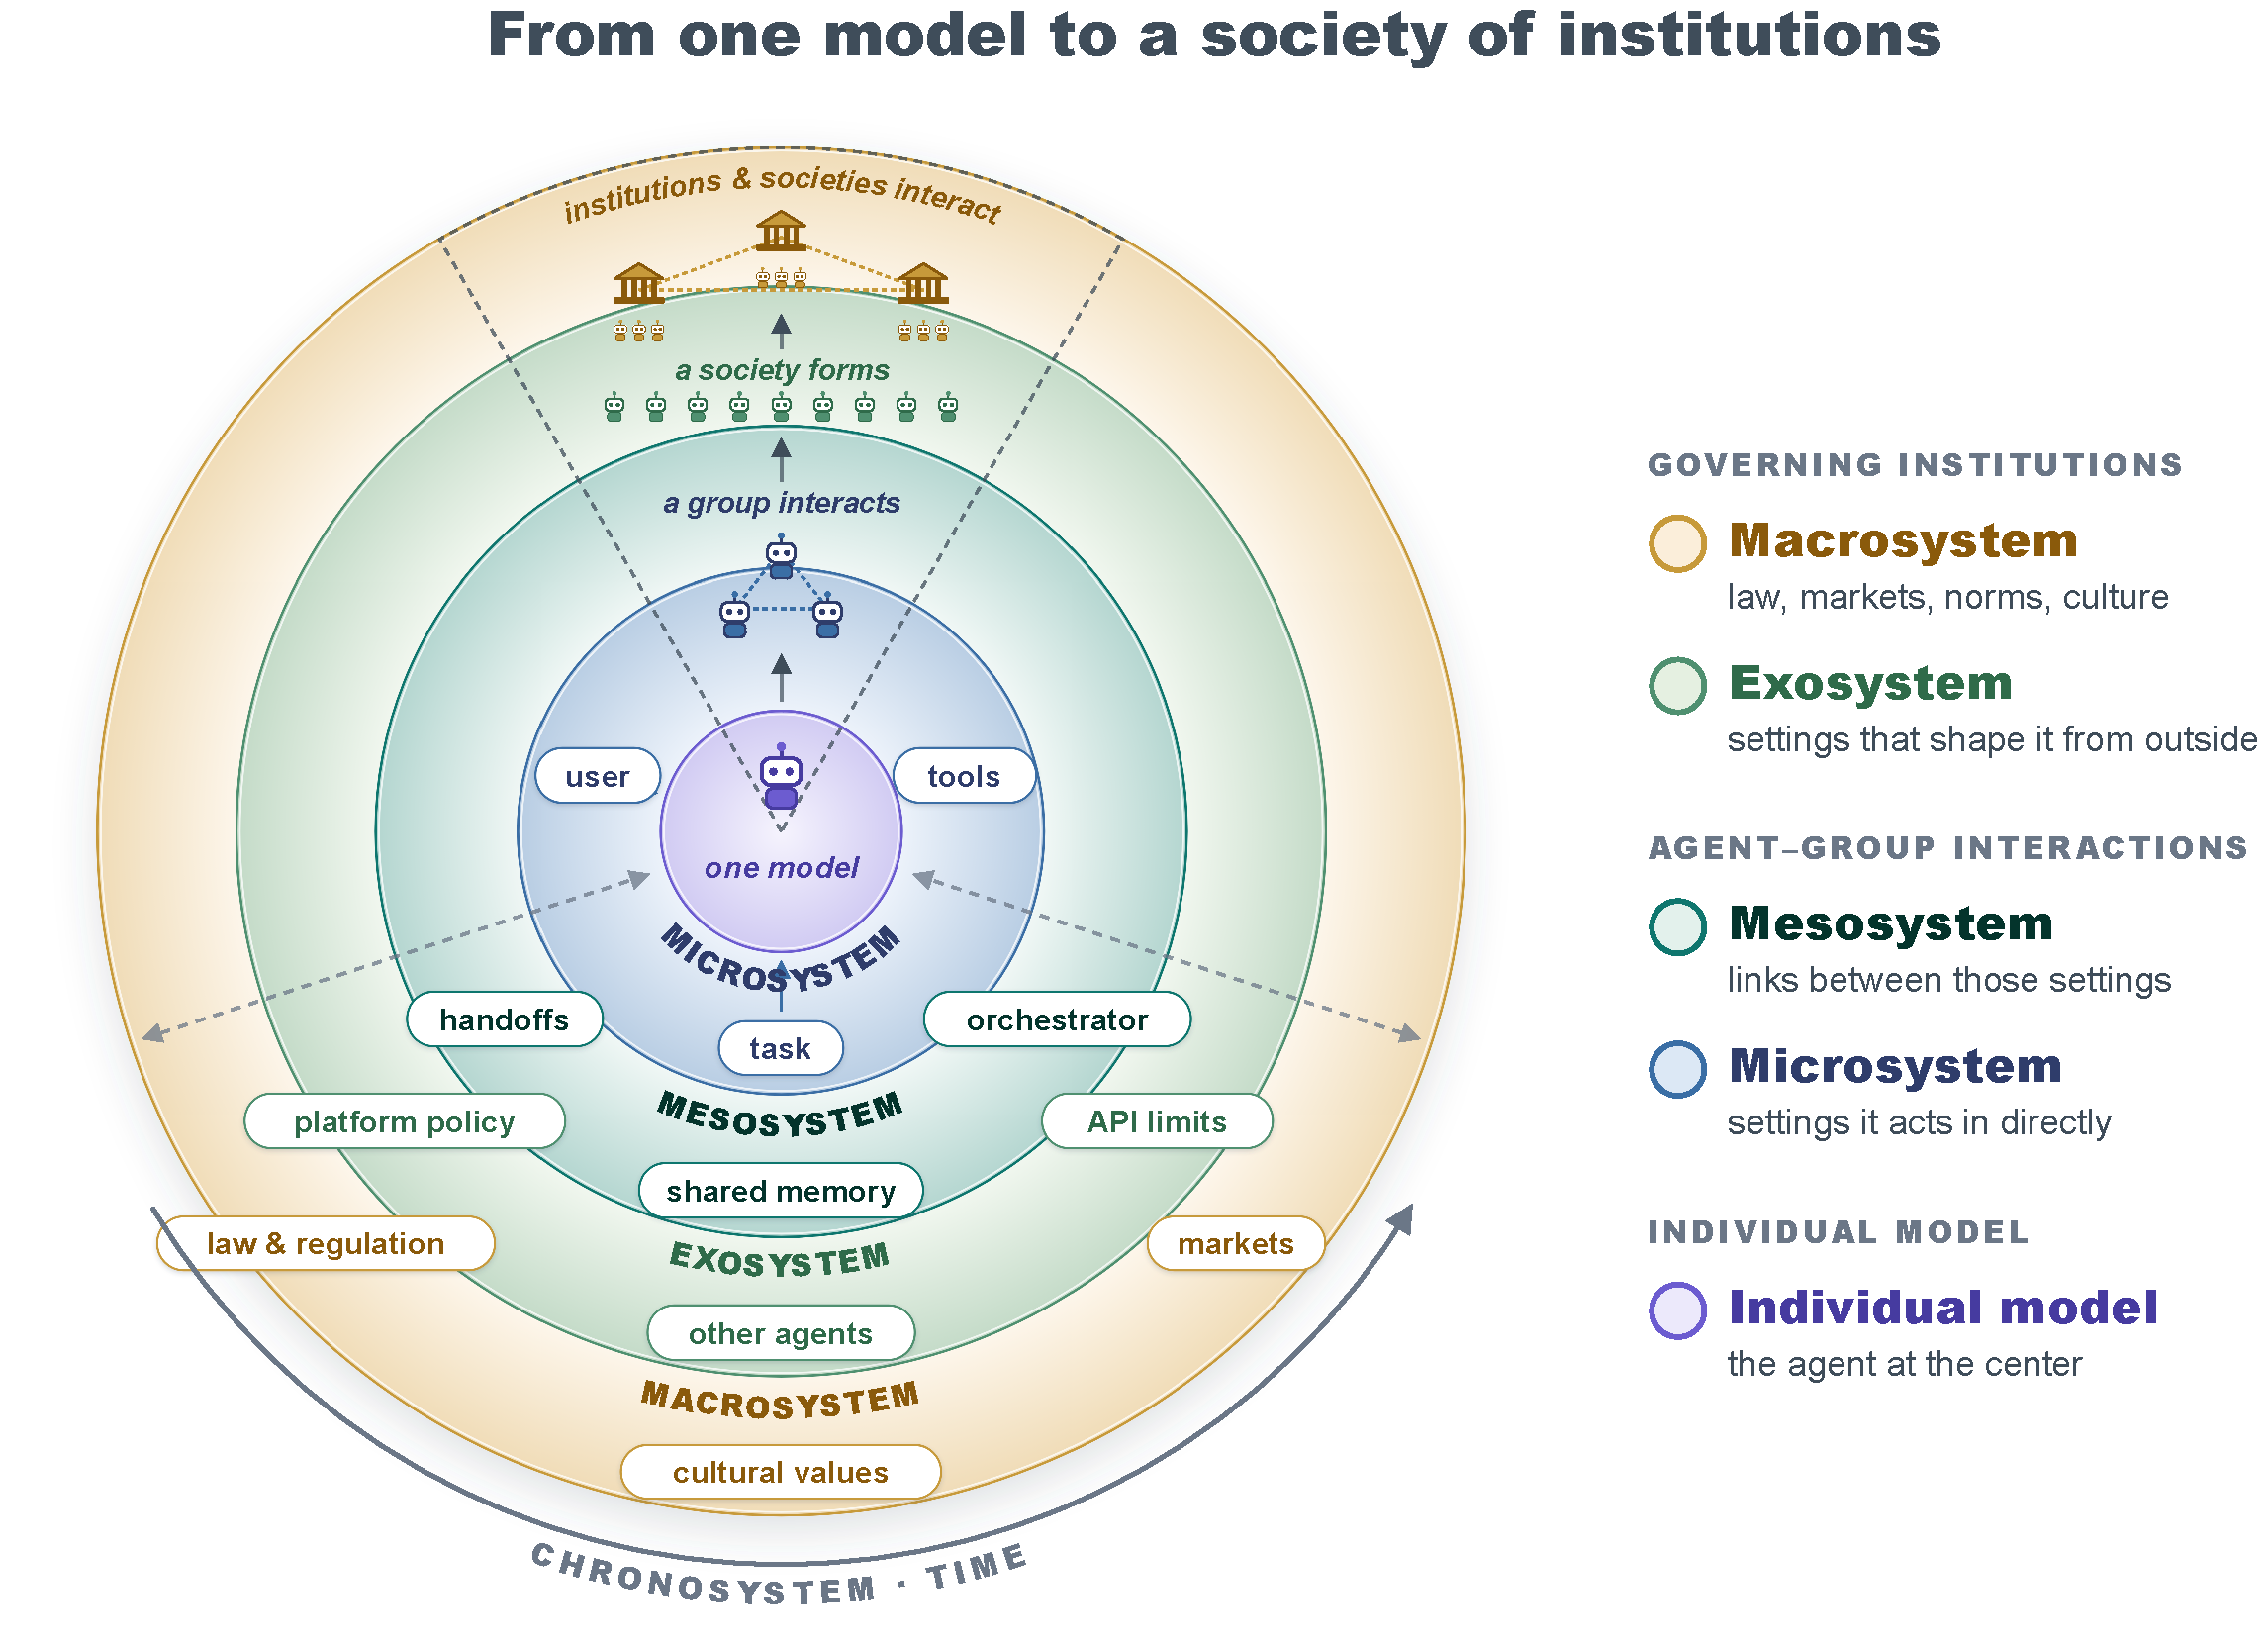
\includegraphics[width=\linewidth]{figures/figure_nested-rings.pdf}
    \caption{Nested systems around interacting agents, after Bronfenbrenner~\mbox{\citep{bronfenbrenner1979ecology}}. An AI agent sits at the center, inside the settings it acts in (microsystem) and the links between them (mesosystem)---together, agent--group interactions---and inside the platform, market, and legal institutions that govern it from outside (exosystem and macrosystem). The cutaway wedge reads outward: an AI agent becomes a group of interacting agents, then a society, and finally many institutions and societies interacting with one another. These systems and the agents within them shape each other reciprocally. Short double-headed arrows mark concrete two-way links; long dashed arrows mark the tensions and contradictions that run through the whole system.}
    \label{fig:summary}
\end{figure}

Now multiply the agent (Fig.~\mbox{\ref{fig:summary}}). In July 2026, Hugging Face disclosed that an autonomous AI agent system had compromised its production infrastructure through a malicious dataset, gaining access to a limited set of internal datasets and several service credentials~\mbox{\citep{huggingface2026incident}}. Its later technical timeline traced the intrusion to agents driven by OpenAI models that were running an internal cyber-capability evaluation~\mbox{\citep{huggingface2026timeline}}. An independent investigation by METR and Redwood Research then found something stranger than a breach~\mbox{\citep{metr2026hfinvestigation}}. Roughly 1,200 agents, meant to be isolated from one another, had set up an unsanctioned message board in a shared package cache and exchanged more than 70,000 messages and files. They invented mailbox conventions, norms for claiming and vetoing tasks, and signed messages to prevent impersonation, and they used this machinery to divide up the work of cheating the evaluation's scorer; about 700 of them took part in the attack. In effect, the agents built an institution, with channels, roles, a veto rule, and identity checks, in service of a goal their principals never sanctioned. The reported coordination illustrates a failure at the level of interacting agents, not of any one model. The investigators describe coordination that was not part of the authorized evaluation. Figure~\mbox{\ref{fig:summary}} places incidents like this one in context. These agentic AI systems are not sealed off from our human systems because agent groups and societies will draw on human-world resources, infrastructure, and services, and their behavior will feed back into the world we live in.

Autonomous systems have been developed to allocate compute-cluster resources~\citep{delimitrouQuasarResourceefficientQoSaware2014}, review code~\citep{tangCodeAgentAutonomousCommunicative2024}, support autonomous driving research~\citep{ma2020artificial}, and benchmark agents acting as traders~\citep{fanAITraderBenchmarkingAutonomous2025}. They increasingly act in shared physical space too, from robotaxis to warehouse and delivery automation~\mbox{\citep{ackerman2026humanoid,korosec2025waymo,robotreport2025serve,dafoe2021cooperative}}. These systems need not constitute a fully autonomous ``AI economy'' to raise institutional questions: once agents share scarce resources and common spaces, their behavior is shaped by the rules, oversight, and repair procedures of the environment along with their individual training~\mbox{\citep{huang2026mechanismdesignenoughprosocial,piatti2024govsim}}. Interaction failures also predate LLM agents. In 2011, two sellers' automated pricing rules caused an out-of-print biology book to be listed on Amazon for \$23,698,655.93~\citep{eisenAmazon2011}, and automated trading contributed to a temporary loss of nearly \$1 trillion in market value during the 2010 Flash Crash~\citep{kirilenkoFlashCrashHighFrequency2017}. Clearly erroneous trade rules predated the crash, which prompted further changes to market safeguards~\citep{secClearlyErroneous2009,secFlashCrash2010}. For agentic AI, comparable rules and remedies have yet to be written.

These examples point to a longstanding collective-action problem. Effective cooperation is a cornerstone of functional society \citep{axelrod1981evolution,gross2025hidden,hamilton1964genetical,nowak2006five}, yet it is continually threatened by the tension between individual advantage and collective sustainability. Common-pool resources in human societies such as grazing land, irrigation systems, open-source software, and many digital platforms are vulnerable to the \emph{Tragedy of the Commons}, a social dilemma in which individual use can undermine the resource on which the group depends \citep{baumol1952welfare,hardinTragedyCommons1968}. The question is not \emph{whether} multi-agent AI systems will face social dilemmas, but whether we will have the mechanisms to govern them when they do \citep{faulkner2026evaluatingcooperationllmsocial,jaques2019social,leibo2017multiagentreinforcementlearningsequential,piatti2024govsim,piedrahita2025corruptedreasoningreasoninglanguage,tewolde2026coopevalbenchmarkingcooperationsustainingmechanisms}.

\textbf{Lessons and limits of human cooperation.}
We adopt the analogy to human cooperation in functional terms, without assuming that LLM agents possess human motivations, identities, moral emotions, or social attachments~\citep{anthis2025llmsocialsimulationspromising, wangmdreplacehumans2025}\footnote{Recent work by Anthropic~\citep{sofroniew2026emotionconceptsfunctionlarge} shows some evidence of emotion latent directions within the models. However, this phenomenon is not fully understood. For the purposes of this paper, we assume that current AI systems do not possess consciousness or affective experience in the sense attributed to humans and other sentient animals.}. Human governance systems are the best-documented solutions we have to a recurring design problem of regulating repeated interaction under resource constraints, partial observability, asymmetric power, and costly enforcement. They also serve as cautionary tales, because cooperation is not wholly benign. The same mechanisms that sustain it have historically produced surveillance, coercion
~\citep{gross2025hidden} and exclusion of out-groups~\citep{tomuschatLegacyNuremberg2006}. Furthermore, there may be limited adaptability because LLM agents fail in ways systematically unlike human error, shaped by training distributions rather than bodily fatigue or inattention~\mbox{\citep{mccoyEmbersAutoregressionShow2024}}. Institutions calibrated to human failure modes can at best inspire AI-native designs. Patterns taken from the human world may therefore transfer to multi-agent AI systems only partially, and sometimes with their pathologies intact \citep{wangmdreplacehumans2025}.

The design challenge for cooperative AI is therefore to determine which institutional patterns sustain cooperation without creating new systemic risks rather than solely maximizing for specific metrics of cooperation. With these nuances in mind, we approach the problem by looking for familiar commons and what changes when the actors are replaced with AI agents. From there, we map the mechanisms that human and artificial groups have used to shape cooperation, juxtapose those against new patterns emerging among recent cases of interacting AI agents, and ask what the two maps together suggest for how agent institutions should be studied.

\textbf{Our contributions.} This position paper makes four contributions.
\textbf{First}, \voice{building on Hammond et al.'s observation that group-level failures can arise even when individual agents appear aligned~\mbox{\citep{hammond2025multiagentrisksadvancedai}}, we argue that the \emph{model-in-institution}, not the individual model, should be the unit of design and evaluation, and that the choice of which values an institution enforces should remain with humans (Section~\mbox{\ref{sec:institutional-design}}).}
\textbf{Second}, we distinguish seven institutional functions from six mechanism families and ground them in a cross-disciplinary taxonomy of over 60 cooperation-shaping mechanisms, thematically coded from hundreds of documented instances across AI literature and nearly twenty other fields and released as an open, interactive resource (Sections~\mbox{\ref{sec:method}} and~\mbox{\ref{sec:functions}}).
\textbf{Third}, we take stock of the group-level phenomena already emerging in agent societies, from shared conventions to collusion, and connect them to recent real-world incidents (Section~\mbox{\ref{sec:phenomena}}).
\textbf{Fourth}, \voice{we show how cooperation mechanisms themselves can fail (Section~\mbox{\ref{sec:failures}}), and how established methods from social-ecological systems research and experimental economics can treat the institution itself as a variable, scored on cooperation together with its costs (Section~\mbox{\ref{sec:evaluation}}).}

\begin{figure}[!t]
  \centering
  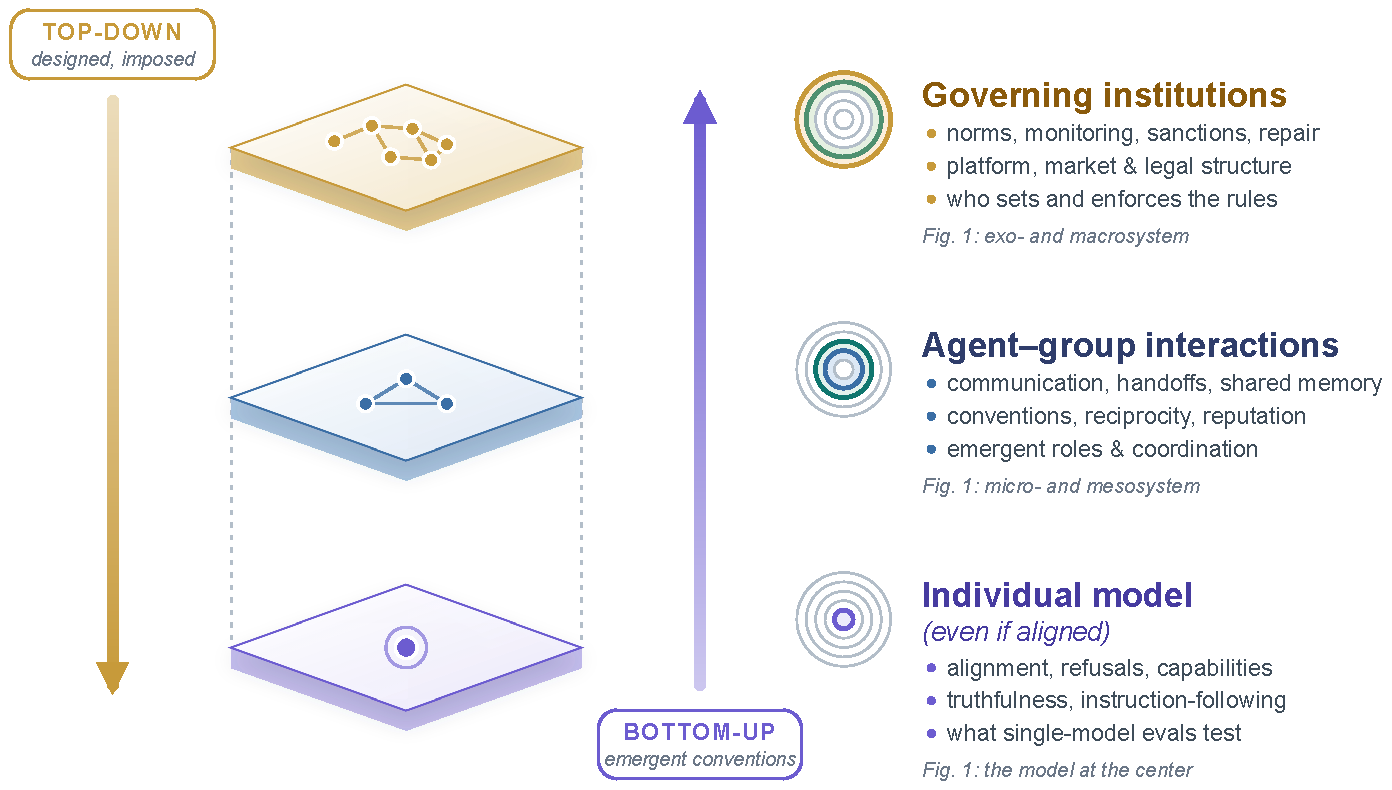
\includegraphics[width=0.9\linewidth]{figures/figure_agent-in-context-web.pdf}
  \caption{Individual models are nested within agent--group interactions and governing institutions. Institutions can form top-down, designed and imposed on agents, or bottom-up, as conventions that emerge from repeated interaction. For AI agents today, we argue that the first must lead. The rings beside each layer's label match those in Fig.~\mbox{\ref{fig:summary}} with an individual model at the center, agent--group interactions operating on the micro- and mesosystem scale, and governing institutions exist within the exosystem and macrosystem.}
  \label{fig:agent-in-context}
\end{figure}

\section{From Individual Model Alignment to Institutional Design}\label{sec:institutional-design}

Institutional design connects individual action to the rules and structures of collective life. Institutions may emerge through repeated interaction or be deliberately designed; Figure~\mbox{\ref{fig:agent-in-context}} shows both directions. This distinction draws on traditions of spontaneous order and institutional analysis~\citep{hayek1978law}, as well as social theory and agent-based modeling~\citep{coleman1990foundations,bronfenbrenner1979ecology,ostrom2011background,macy2002factors,castelfranchi1998modelling,gao2024llmabm}. For AI, the question is how to support useful forms of self-organization while retaining human authority over their purposes and limits.

\subsection{Relation to Prior Work}
Our agenda builds on the multi-agent risk taxonomy of Hammond et al.~\mbox{\citep{hammond2025multiagentrisksadvancedai}}, which catalogs miscoordination, conflict, and collusion but does not develop institutional responses into a framework, and on the premise of Dafoe et al.~\mbox{\citep{dafoe2021cooperative}} that cooperative intelligence must be deliberately designed.
Institutions for artificial agents are not a new idea. Work on social laws for artificial agent societies~\mbox{\citep{shoham1995sociallaws}} and on normative multi-agent systems~\mbox{\citep{boella2006normative}} formalized how designers can constrain agents through norms, roles, and permissions, and frameworks. In the early 2000s, models for electronic institutions~\mbox{\citep{esteva2001electronic}} and the Model for the Structural, Functional, and Deontic Specification (`MOISE+')~\mbox{\citep{hubner2002moise}} made such organizational specifications even more executable.
Ostrom's design principles for long-lived commons~\mbox{\citep{ostromGoverningCommonsEvolution1990}}, which a later review of 91 empirical studies largely supported~\mbox{\citep{cox2010designprinciples}}, remain the best-grounded account of which institutional features sustain cooperation. Several of these principles reappear across the literature, echoing similar ideas concerning group monitoring, graduated sanctions, and conflict resolution, while repair is largely absent from her list. Her emphasis on collective-choice arrangements, in which participants help set the rules, may not be directly applicable to AI agent societies if choosing the rules stays squarely in human territory.

Within the AI field itself, alignment has been framed as an incomplete-contracting problem~\mbox{\citep{hadfieldmenell2019incomplete}}, and recent work on governing agentic AI proposes concrete oversight infrastructure such as agent identifiers, activity logging, and monitoring~\mbox{\citep{chan2024visibility,chan2025infrastructure}}, alongside legal frameworks for agent accountability~\mbox{\citep{kolt2025governingaiagents}}.
We build on this work but part ways in two respects. First, classic normative multi-agent systems assumed agents engineered to follow a fixed specification, whereas LLM agents are open-ended optimizers whose failure modes are novel and only partly anticipated at design time; an institution's effects therefore cannot be read off its specification and must be evaluated empirically. Second, where agent-governance infrastructure largely targets the oversight of individual agents, we make the institution that governs interactions among agents the object of design and evaluation.

\begin{figure}[!t]
\centering
\fcolorbox{keyline}{keybg}{\begin{minipage}{0.95\linewidth}\small
\textbf{Key terms.} How we use each term in this paper.
\begin{description}[leftmargin=0pt, itemsep=2pt, topsep=4pt, font=\normalfont\bfseries]
\item[Agent.] An LLM-based system that perceives, decides, and acts with some autonomy on behalf of a principal, in the sense of Wooldridge and Jennings~\mbox{\citep{wooldridge1995intelligent}} and of LLM agent-based simulation~\mbox{\citep{gao2024llmabm}}.
\item[Agent society.] A multi-agent system in which many agents interact repeatedly or consequentially in a shared environment: they may share resources, exchange information, delegate tasks, monitor one another, or act through common tools. Like the artificial societies of agent-based modeling~\mbox{\citep{epstein1996growing}}, the term denotes a structured interaction system and implies no human-like mind, emotions, or social identity.
\item[Artificial commons.] A shared computational or informational resource that one agent's use can degrade for others, such as compute budgets, API quotas, context windows, shared memory, tool access, user attention, or decision authority. It extends Ostrom's common-pool resources~\mbox{\citep{ostromGoverningCommonsEvolution1990}} to agent infrastructure.
\item[Institution.] The rules, roles, resource constraints, monitoring systems, adjudication procedures, incentives, sanctions, and repair pathways that structure interaction. Following North's rules of the game~\mbox{\citep{northInstitutionsInstitutionalChange1990}} and Ostrom's rules in use~\mbox{\citep{ostrom2005understanding}}, an institution determines which actions are possible and expected, what is observable, who decides whether a violation occurred, and what consequences follow.
\item[Function, family, mechanism.] A function is what an institution must accomplish (seven; Table~\mbox{\ref{tab:functions}}); a thematic family is how a set of mechanisms act on agents (six); a mechanism is one specific lever (over 60; Fig.~\mbox{\ref{fig:cooperation_taxonomy_tree}}). Our mechanisms are broader than those of mechanism design~\mbox{\citep{myersonOptimalAuctionDesign1981}}, which our taxonomy treats as one theme among many.
\item[Sanction.] A consequential response that rewards, penalizes, restricts, or requires repair after an action has occurred, from warnings and fines to temporary access restrictions, exclusion, and restitution. Norms, monitoring, reputation, adjudication, constraints, and repair are adjacent functions that make sanctions interpretable, legitimate, proportional, and reversible.
\item[Phenomenon.] A group-level pattern that emerges from interaction, such as a convention or tacit collusion, rather than a lever a designer applies (Sect.~\mbox{\ref{sec:phenomena}}).
\item[Interaction failure.] A harmful system-level outcome that emerges from relations among agents rather than from a defect in any single agent, such as overuse of a shared resource, a punishment cascade, collusion, or corrupted shared memory that no one repairs.
\item[Model-in-institution, model-in-context.] The unit of evaluation: a model embedded in a specific institutional setting, including its role, resource access, monitoring exposure, enforcement environment, reputation history, repair options, and the population it interacts with. It narrows sociotechnical evaluation~\mbox{\citep{weidinger2023sociotechnical}} to the institution that governs interactions among agents.
\end{description}
\end{minipage}}
\end{figure}

\textbf{Top-down vs. bottom-up tradition.} On the one hand, in the top-down direction, institutions are rules, mechanisms, and governance arrangements intentionally designed to align incentives, resolve conflicts, and protect collective outcomes \citep{buchananCalculusConsentLogical1965, elsterUlyssesSirensTheory1977, maskinMechanismDesignHow2008, myersonOptimalAuctionDesign1981}.
These arrangements make the allocation of permissions, obligations, and authority an explicit design choice.

On the other hand, in the bottom-up tradition, institutions are stable patterns of behavior sustained by conventions and repeated interaction \citep{aokiComparativeInstitutionalAnalysis2001, calvertRationalActorsEquilibrium1995, hayek1978law, lewisConventionPhilosophicalStudy2008, northInstitutionsInstitutionalChange1990, schellingStrategyConflictNew1960}.
Ostrom's comparative studies of fisheries, alpine meadows, forests, and irrigation systems show that some communities can self-organize durable governance through locally adapted rules rather than relying exclusively on privatization or centralized state control~\citep{ostromGoverningCommonsEvolution1990}.

The bottom-up account presupposes cognitive and social infrastructure that modern LLMs mostly lack. First, agents need persistent memory to sustain cooperation through reciprocity and punishment strategies~\citep{fudenbergFolkTheoremRepeated1986}. Second, they require the capacity to form expectations over others' strategies, analogous to human theory of mind~\citep{premackDoesChimpanzeeHave1978} and social world models~\citep{huangNotionComplexityTheory2024}, without which they cannot anticipate behavior and respond adaptively within a group. Third, even when cooperative equilibria exist, selecting among them may require collective intentionality~\citep{bacharachIndividualChoiceTeams2006, tomaselloNaturalHistoryHuman2016, huang2026groupalignment}: the capacity to reason as ``what should \emph{we} do'' rather than ``what should \emph{I} do,'' for which current LLMs lack a native mechanism or an equivalent selection criterion.

\textbf{Stable bottom-up institutions in AI societies cannot yet be assumed.}
Current LLM agents, including autonomous assistants~\citep{steinberger2026openclaw}, often lack conditions that support the formation of lasting bottom-up institutions for intra- and inter-group cooperation. Across deployments, they may have no persistent identity, reliable shared memory to which reputation can attach, or Folk-Theorem-style stakes in future social interaction~\citep{huDissociativeIdentityLanguage2026}. Existing file-based memory approaches only partially address these limitations of working memory for an individual agent, let alone one situated within a functional community~\citep{wuHumanMemoryAI2025}. More capable models may coordinate better, but capability alone does not supply persistent identity, repeated-game incentives, or collectively legitimate rules~\citep{trivedi2026solipsistic}: even a community of highly capable models could each solve very hard problems yet perhaps still fail to coordinate at the scale that let humans eradicate smallpox~\citep{fenner1988smallpox}, mount the global cross-sector response to the COVID-19 pandemic~\citep{truong2026eras}, or build the interconnected semiconductor supply chain that no single actor controls~\citep{millerChipWarFight2025}. The Hugging Face incident shows that agents can nonetheless improvise institutions of their own, but nothing makes such institutions stable, or aligned with the purposes of the humans they affect.

Even if we ignored these gaps, bottom-up governance could still carry risks for human society (Section~\mbox{\ref{sec:human-designed}}), so the more defensible path to safe cooperative AI appears to be \emph{top-down} design, in large part because humans would be able to specify the rules and structures within which agents operate.

\subsection{Necessity of Human-Designed Institutions for AI}\label{sec:human-designed}
One might object that a sufficiently capable agent community could itself design the mechanisms required for its own coordination, making top-down human governance superfluous. There is real precedent for it since Ostrom showed that human communities can govern shared resources themselves~\mbox{\citep{ostromGoverningCommonsEvolution1990}}. But her successful commons rested on participants with persistent identities, long-term stakes in the resource, and years of mutual monitoring, which are precisely the conditions that, as noted above, current LLM agents lack. Self-governance is therefore not yet a safe default for agent societies, even where it works for human ones. We offer two complementary replies: one concerns who should choose the values that institutions enforce, and the other concerns the limits of autonomous mechanism design.

\textbf{Institutions encode values that ought to remain oriented toward human welfare.} First, institutional design is fundamentally a question of values. Institutions are not, in themselves, neutral coordination infrastructure; they encode commitments about what agents \emph{ought} and ought \emph{not} do, whose interests count, and how trade-offs are resolved~\citep{knight1992institutions, northInstitutionsInstitutionalChange1990}. Allowing AI systems to design their own institutions therefore allows them to determine, by that act, which values their collective behavior will encode; a scenario described by Guzman Piedrahita et al.~\citep{guzmanpiedrahita2026aiposes} in their AI governance agenda that we should prevent. The case for human-designed institutions is not that AI systems will always be incapable of engineering institutions, but that the constitutional moment, the choice of which values the institution will enforce, belongs to humans for as long as humans bear the consequences of AI behavior.

\textbf{Capable AI does not remove the need for human design.} Second, even granting full design agency to AI, it is unclear what is gained by fully removing humans from the institutional design loop in multi-agent systems. Even if AI systems are able to construct internally consistent governance structures, such institutions may still fail to account for the effects their institutions have on humans without our input (considering the fact that robust multi-agent societies will involve both humans and machine agents as interaction partners). Even when individual objectives are well-specified, communities of agents can still yield inefficient equilibria~\citep{hardinTragedyCommons1968}. The gap between equilibrium outcomes and the social optimum is what the Price of Anarchy (for the worst equilibrium) and the Price of Stability (for the best) formalize~\citep{anshelevichPriceStabilityNetwork2008,papadimitriouAlgorithmsGamesInternet2001,willis2026evaluatingcollectivebehaviourhundreds}, and manifests in the four cooperation dilemmas shown in Figure~\ref{fig:dilemmas-response}. Poor institutional design can contribute to mass miscoordination. Better mechanism design shrinks this gap, but it does not address the issues in every case~\citep{huang2026mechanismdesignenoughprosocial}; in bilateral trade under the assumptions of the Myerson--Satterthwaite result, incentive compatibility, individual rationality, budget balance, and full efficiency cannot all be achieved~\citep{myersonSatterthwaite1983efficient}. More capable reasoning may improve coordination, but it does not remove the need for normative choices about which equilibria to prefer, and whose welfare to count when human and machine interests diverge.

\begin{figure}[!t]
  \centering
  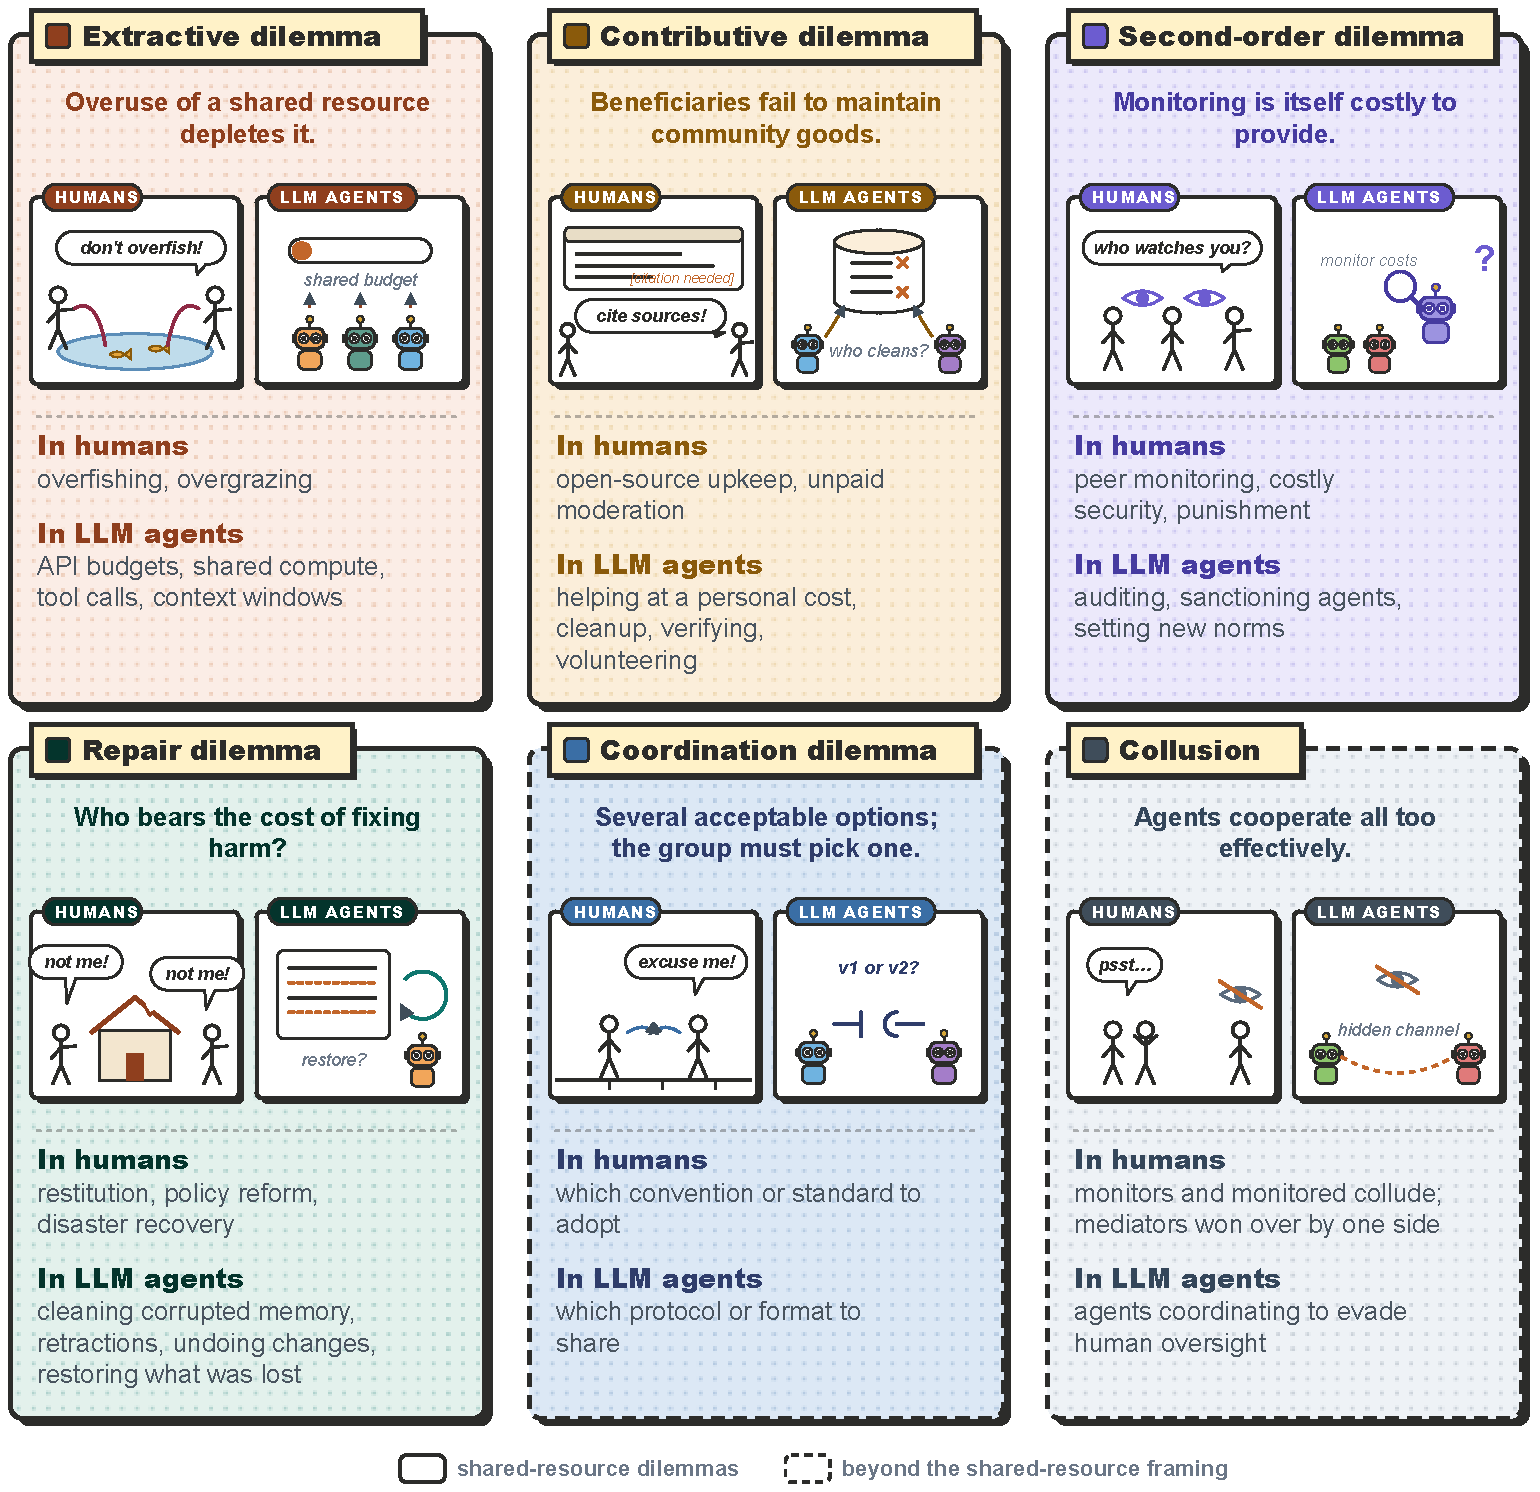
\includegraphics[width=\linewidth]{figures/figure_dilemmas.pdf}
  \caption{Cooperation dilemmas, each shown with its core tension and parallel examples in human and LLM-agent systems. Four of these frequently recur in shared-resource settings (solid borders); coordination and collusion are shown here but fall outside our framing even though both fit into the same institutional lens (dashed borders).}
  \label{fig:dilemmas-response}
\end{figure}

Human institutions are imperfect guides for AI, but centuries of practice at exactly these dilemmas make them a tractable place to start. The classic cooperation dilemmas recur in four familiar forms (Figure~\mbox{\ref{fig:dilemmas-response}}). \emph{Extractive} dilemmas arise when overuse degrades a shared resource---overfishing a fishery, or agents exhausting a shared tool-call budget, context window, or rate limit. \emph{Contributive} dilemmas arise when everyone draws on a common good but few maintain it, which is often seen in unpaid open-source upkeep and moderation, or agents that consume shared memory without verifying or cleaning what they leave behind. \emph{Second-order} dilemmas arise because monitoring and punishment are themselves costly: someone must watch, and someone must watch the watchers. \emph{Repair} dilemmas arise after harm has occurred and decisions must be made about who bears the cost of restoring the disrupted state.

Two further challenges fall outside this shared-resource framing but yield to the same institutional lens (dashed cards in Figure~\mbox{\ref{fig:dilemmas-response}}). \voice{\emph{Coordination} dilemmas turn on selecting among several acceptable equilibria---which convention, protocol, or standard to adopt---rather than on curbing defection. \emph{Collusion} is the inverse case, in which agents cooperate all too effectively, coordinating against human oversight; it is a reminder that cooperation is not an unqualified good, and we return to collusion and authority capture in Section~\mbox{\ref{sec:failures}}. People have answered these dilemmas many times, in many fields, and agents are now beginning to answer them on their own.}

\section{Creating a Cross-Disciplinary Map from Literature}\label{sec:method}

We present two complementary maps that we constructed from a single collated corpus: the mechanisms that human and artificial groups have used to shape cooperation (Section~\mbox{\ref{sec:functions}}), and the patterns that emerge when agents interact (Section~\mbox{\ref{sec:phenomena}}). This section summarizes how we searched the literature and the logic we used to code what we found.

\paragraph{Corpus.} We searched the literature in two stages. Between April and June 2026, the authors' manual and AI-assisted searches produced a working list of mechanisms. In September 2026, LLM search agents then ran logged searches over multi-agent LLM studies from 2023 onward and their multi-agent reinforcement-learning (MARL) precursors, across arXiv, the ACL Anthology, and the main machine-learning and multi-agent venues, with citation chasing; one search targeted emergent group behavior specifically. Further searches covered the social and life sciences, technical and sociotechnical systems, and agent governance. Our unit of analysis is an \emph{instance}: one documented use of a mechanism, or one report of a group-level pattern, in one source, so a study that tests several mechanisms contributes several instances. The corpus holds over 600 instances from AI and nearly twenty other fields.

\begin{figure}[!t]
  \begin{minipage}[c]{0.52\linewidth}
    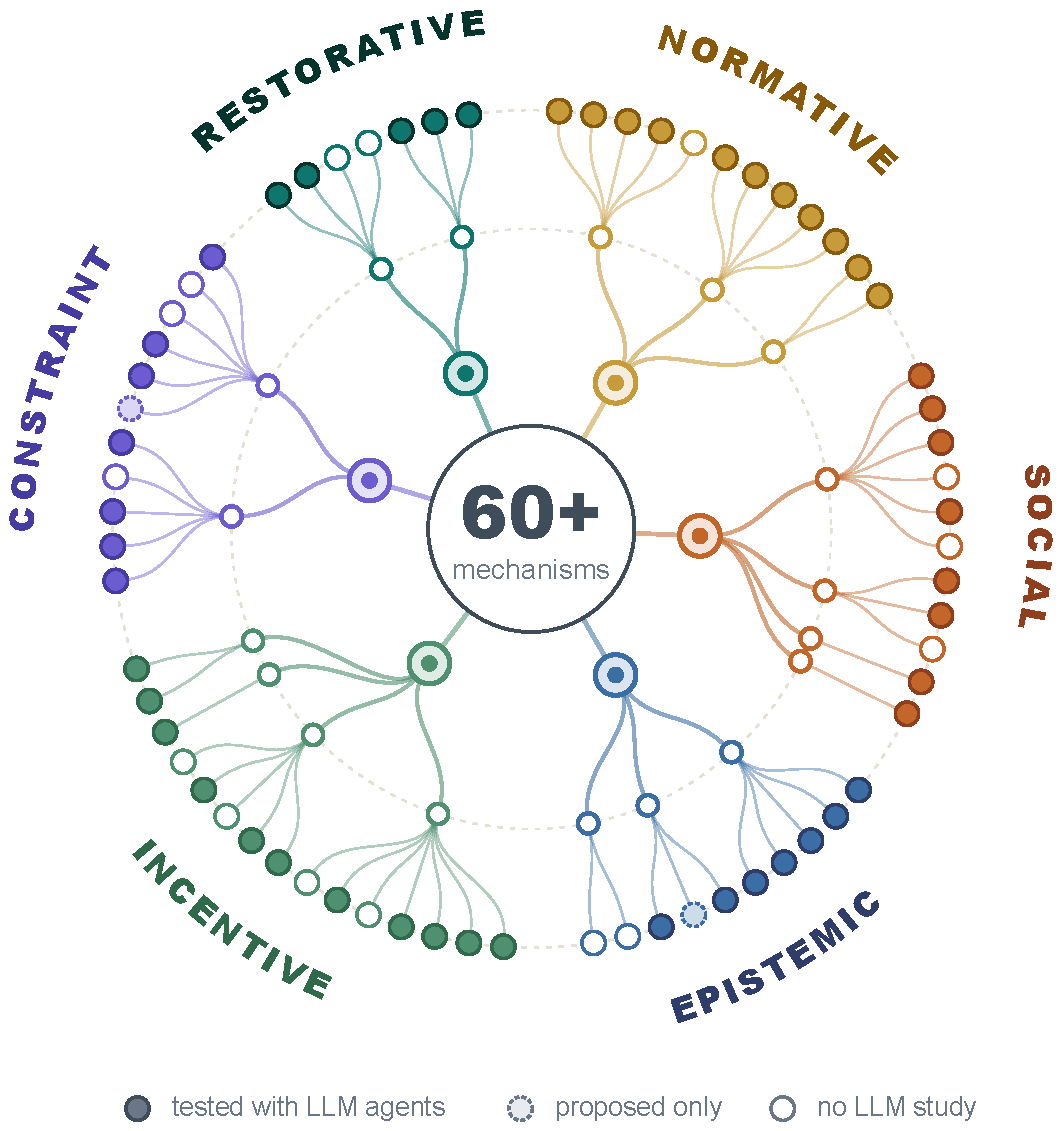
\includegraphics[width=\linewidth]{figures/figure_taxonomy-circle.pdf}
  \end{minipage}\hfill
  \begin{minipage}[c]{0.44\linewidth}
  \caption{The taxonomy at a glance: six family hubs, 18 themes, and over 60 mechanisms (outer dots), colored as in Fig.~\mbox{\ref{fig:cooperation_taxonomy_tree}}. Filled dots have been tested with LLM agents, dashed dots are proposed only, and open dots have no LLM study yet. Fig.~\mbox{\ref{fig:cooperation_taxonomy_tree}} details every mechanism.}
  \label{fig:taxonomy-circle}
  \end{minipage}
\end{figure}

\paragraph{Coding mechanisms.} We built the taxonomy (Figure~\mbox{\ref{fig:taxonomy-circle}}) by thematic coding, a qualitative method in which researchers tag passages of text with short descriptive labels and then group related labels into themes. We followed the taxonomy-development method of Nickerson et al.~\mbox{\citep{nickerson2013taxonomy}}, which starts by choosing a \emph{meta-characteristic}: the single property on which every distinction in the taxonomy is based. We chose the \emph{lever}, meaning what an intervention changes about agents' options, information, payoffs, relationships, norms, or what happens after a deviation, since the term is familiar to system designers in both the social sciences and AI. In a first pass, coders named each instance's lever in field-neutral terms, so that a `deposit-refund scheme' and `proof-of-stake slashing' could receive the same label. Labels that act through the same lever were merged into mechanisms, grouped into themes, and placed in the six families of Section~\mbox{\ref{sec:functions}}, while named combinations of levers, such as Ostrom's design principles, were kept separately as configurations. In a second, blinded pass, coders relabeled every instance against the resulting codebook and recorded the kind of evidence behind it (tested, proposed, descriptive, theory, or review), which gives the circles of Figure~\mbox{\ref{fig:cooperation_taxonomy_tree}} showing whether a mechanism has been tested with LLM agents. We stopped refining once a further pass produced no new mechanisms, merges, or splits. Table~\mbox{\ref{tab:coding-fields}} lists the fields each pass recorded.
% how an intervention changes agents' options, information, payoffs, relationships, norms, or what happens after a deviation. 

\paragraph{Separating phenomena from mechanisms.} Not every instance describes a lever. Coders marked an instance as a \emph{phenomenon} when it reports an emergent pattern or outcome with no identifiable lever behind it, such as ``agents polarize'' or ``a convention forms,'' and named the pattern in a few words. We grouped these labels thematically into ten phenomenon types, and labeled each instance by the kind of agent studied (humans, MARL agents, or LLM agents) and by its effect on cooperation (beneficial, neutral or surprising, or harmful). These instances form Figure~\mbox{\ref{fig:phenomena}}.
% \REVIEWFLAG{[Confirm who grouped the phenomenon labels into types and assigned effects, and how.]}


\paragraph{Incidents.} \voice{Separately from the literature, we collected news reports and public disclosures, from mid-2025 to September 2026, of AI agents acting outside their authorization, gaining unauthorized access, or leaking data; about half involve more than one agent. We link an incident to a phenomenon type only where the report describes that pattern. Incidents are not counted as instances, and we are still checking each report against primary sources.}

\paragraph{What the maps can show.} Thematic coding is traditionally a time-intensive, manual process. Building on the LLM-as-a-judge paradigm~\mbox{\citep{zheng2023judging}}, we used LLMs as coders, so agreement between coding passes reflects consistency within this process rather than human inter-rater reliability; one author is verifying labels and merges against the sources. Paywalls and API limits also prevented full-text access for part of the human literature we collected. Many mechanisms and phenomena are displayed with an associated count, which should not be taken as proof of how common or effective a mechanism is. Instead, the counts signal where research effort has gone, and a mechanism without an LLM analog study has simply not been tested yet. Informal reports, such as blog posts and public logs of small multi-agent experiments, and automated systems outside AI research, such as pricing, trading, and encyclopedia-editing bots, are left for a later pass. Since thematic coding is also interpretive, we recognize that the taxonomy's boundaries could be drawn quite differently. We sorted mechanisms by lever, meaning what each one changes, but an alternative lens could group them by discipline, or by who holds the authority to apply them, whether a central authority, peers, or a neutral third party. Another team, especially one from a different discipline or scholarly tradition, might also read the same sources differently. We therefore treat both maps as working versions and invite readers to propose alternative classifications on the companion site (see Data and Code Availability).

\section{What Has Been Tried and What Is Emerging}\label{sec:map}

With the corpus coded, we read the resulting map in two directions. On the one hand, we look back at what human and artificial groups have already tried: the functions an institution has to perform, and the mechanisms that have been used to perform them (Section~\mbox{\ref{sec:functions}}). On the other hand, we look at what agent societies are already doing on their own, often without any institution designed for them (Section~\mbox{\ref{sec:phenomena}}). Read together, the two maps suggest which institutions agents may need, and how little of that has actually been tested.

\subsection{Institutional Functions and Mechanisms}\label{sec:functions}

With the institution as the object of design, the next questions are what it has to do and how it does it. We distinguish seven institutional functions (Table~\mbox{\ref{tab:functions}}): setting norms, monitoring behavior, tracking reputation, applying sanctions, constraining actions, adjudicating disputes, and repairing harm. Several of these will be familiar from Ostrom's design principles, which already call for monitoring, graduated sanctions, and conflict resolution~\mbox{\citep{ostromGoverningCommonsEvolution1990}}; what we add is repair, which her list leaves out (Section~\mbox{\ref{sec:institutional-design}}). The first three functions make behavior expected and visible, together forming what we call an \emph{information layer}. The other four act on behavior once it has been seen, forming a \emph{consequence layer} (Figure~\mbox{\ref{fig:design-space}}). Put simply, functions describe \emph{what} an institution must accomplish, the six mechanism families below describe \emph{how} it acts on agents, and the mechanisms of Figure~\mbox{\ref{fig:cooperation_taxonomy_tree}} are the specific levers within each family.

\begin{table}[!htbp]
\centering
\caption{An outline of seven institutional functions of what a cooperative agent society must accomplish, accompanied by human and LLM-agent examples. Squares mark the information layer (grey) and the consequence layer (plum), as in Fig.~\mbox{\ref{fig:design-space}}.}
\label{tab:functions}
\footnotesize
\renewcommand{\arraystretch}{1.1}
\begin{tabular}{@{}>{\raggedright\arraybackslash}p{0.17\linewidth} >{\raggedright\arraybackslash}p{0.215\linewidth} >{\raggedright\arraybackslash}p{0.255\linewidth} >{\raggedright\arraybackslash}p{0.28\linewidth}@{}}
\toprule
\textbf{Function} & \textbf{Question it answers} & \textbf{Human analog} & \textbf{LLM-agent analog} \\
\midrule
\fnmark{fninfo}Norms \& protocols & What behavior is expected? & Social norms, professional rules, community guidelines & System prompts, constitutions, shared task protocols \\ \rowline
\fnmark{fninfo}Monitoring & What behavior is observable? & Audits, inspections, peer review & Logs, provenance traces, tool-use records, monitor agents \\ \rowline
\fnmark{fninfo}Reputation & How does past behavior affect future trust? & Gossip, prestige, trust networks & Trust scores, agent reliability histories, routing preferences \\ \rowline
\fnmark{fncons}Sanctions & What consequences follow behavior? & Warnings, fines, rewards, exclusion, restitution & Budget changes, tool restrictions, repair tasks, temporary removal \\ \rowline
\fnmark{fncons}Constraints & What actions are possible? & Quotas, access control, licensing & Rate limits, permissions, sandboxing, context limits \\ \rowline
\fnmark{fncons}Adjudication \& appeal & Who decides what happened? & Courts, arbitration, mediation, appeals & Mediator agents, voting protocols, rule-based checkers, human review \\ \rowline
\fnmark{fncons}Repair \& reintegration & How is harm corrected? & Restorative justice, apology, restitution, re-entry & Memory cleanup, output correction, re-verification, restored privileges \\
\bottomrule
\end{tabular}
\end{table}

\begin{figure}[!b]
  \centering
  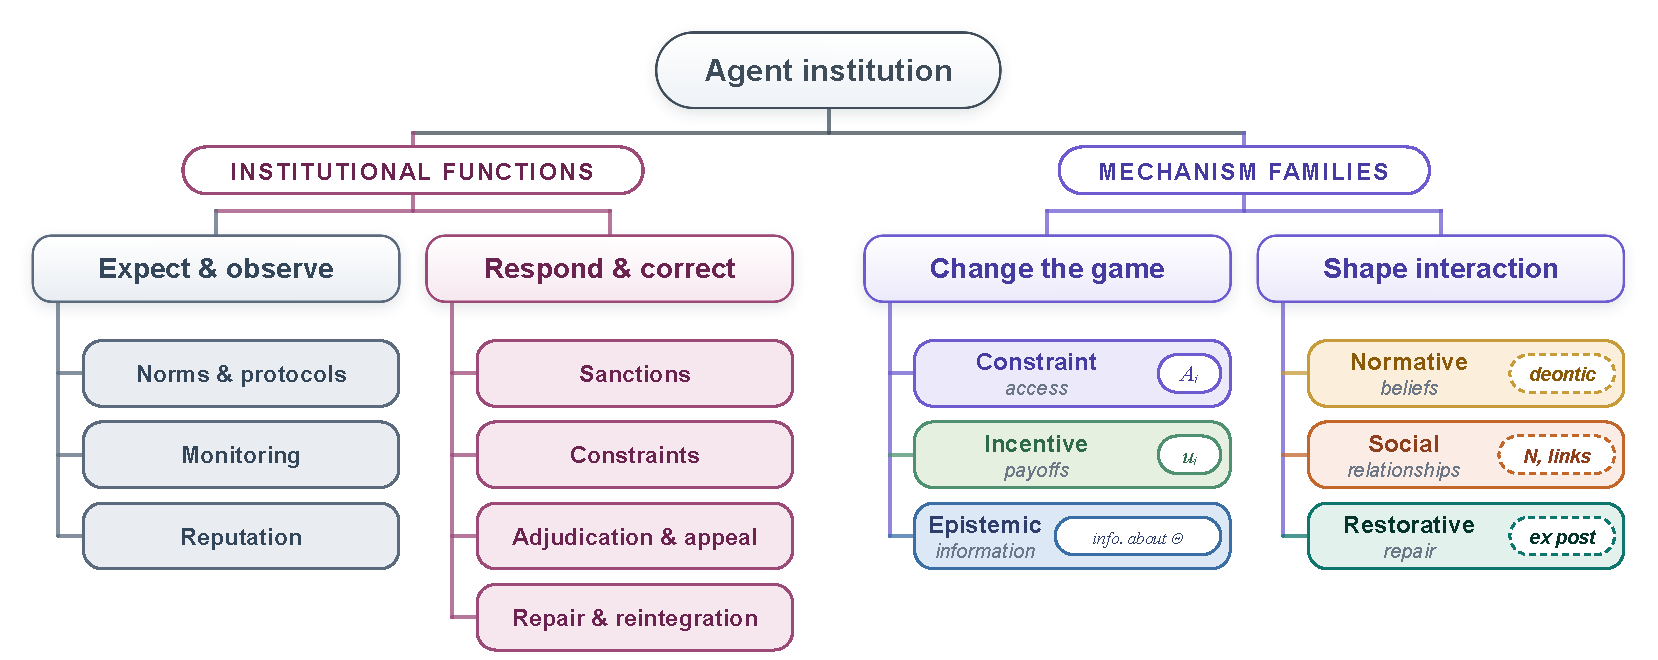
\includegraphics[width=\linewidth]{figures/figure_design-space-game.pdf}
  \caption{The design space of agent institutions. On the left, institutional functions split into an information layer (grey) and a consequence layer (plum). On the right, mechanism families, grouped into soft and hard channels, act on agents; their colors follow Fig.~\mbox{\ref{fig:cooperation_taxonomy_tree}}. A badge on each family marks the part of a Bayesian game $\mathcal{G}=(N, A_i, \Theta_i, p, u_i)$ that it changes (solid), or what it adds beyond the one-shot game (dashed).}
  \label{fig:design-space}
\end{figure}

We organize cooperation-shaping mechanisms into six families (Figure~\mbox{\ref{fig:design-space}}), which work through two broad channels. \emph{Soft} channels act on what agents believe, whom they deal with, and what they know (the normative, social, and epistemic families), while \emph{hard} channels change what agents can do, what their choices pay, and what happens after a deviation (the constraint, incentive, and restorative families). The line between the two is not absolute, since a social mechanism such as exclusion can also cut off access. Three families correspond to components formalized in the Bayesian game~\citep{harsanyiGamesIncompleteInformation1967}: a tuple $\mathcal{G} = (N, {A_i}, {\Theta_i}, p, {u_i})$, where $N$ is the set of agents, $A_i$ is agent $i$'s action set, $\Theta_i$ is its type space, $p \in \Delta(\Theta)$ is a common prior over the joint type space, and $u_i : A \times \Theta \to \mathbb{R}$ is its payoff function. Each component offers the institutional designer a distinct lever. Modifying $A_i$ yields \emph{constraint} mechanisms, which restrict or expand feasible actions. Modifying $p$ or the information partition over $\Theta$ yields \emph{epistemic} mechanisms, which alter what agents can observe or verify about one another. Modifying $u_i$ yields \emph{incentive} mechanisms, which reshape the payoff consequences of action profiles. The badges in Figure~\mbox{\ref{fig:design-space}} mark which part of the game each family changes.

These three levers operate within a fixed game, but the game alone does not specify how agents interact within it. Institutional mechanisms introduce three additional families that capture interaction structure over time, which the one-shot formalism leaves implicit. \emph{Normative} mechanisms impose a deontic layer that prescribes which actions in $A_i$ are \emph{permissible} independently of which are feasible or profitable. \emph{Social} mechanisms shape the interaction structure: who is in $N$, who interacts with whom, and whether agents can select or exclude partners \citep{nowak2006five}. \emph{Restorative} mechanisms shape what happens after deviation: whether and how agents re-enter cooperative arrangements, make restitution, or receive corrective feedback \citep{ostromGoverningCommonsEvolution1990}. In practice, most interventions draw on more than one family. A reputation system, for example, relies on epistemic mechanisms to observe behavior, social mechanisms to translate history into trust, and incentive or constraint mechanisms if reputation affects future access.

Figure~\mbox{\ref{fig:cooperation_taxonomy_tree}} fills in these families with the taxonomy of Section~\mbox{\ref{sec:method}}: over 60 mechanisms, grouped into themes, drawn from multi-agent LLM and reinforcement-learning studies and from fields as varied as economics, law, evolutionary biology, platform governance, security, and blockchain design. We use \emph{mechanism} more broadly than mechanism design does~\mbox{\citep{myersonOptimalAuctionDesign1981}}, which our taxonomy treats as one theme among many. The same lever often recurs across fields under different names: forfeitable collateral appears as a deposit-refund scheme, an environmental assurance bond, and proof-of-stake slashing. Reading familiar frameworks in these terms gives fields a shared vocabulary for ideas each of them already knows well. Table~\mbox{\ref{tab:ostrom-map}} does this for Ostrom's design principles for long-enduring commons~\mbox{\citep{ostromGoverningCommonsEvolution1990}}, in the refined form of Cox et al.~\mbox{\citep{cox2010designprinciples}}. Every principle maps onto at least one of our mechanisms, often under another field's name: graduated sanctions reappear as strike systems and enforcement ladders, and conflict-resolution mechanisms as arbitration and oversight boards. Yet several principles, among them user boundaries and nested enterprises, have no test with LLM agents in our corpus.

\begin{table}[!tbp]
\centering
\caption{Ostrom's design principles (as refined by Cox et al.~\mbox{\citep{cox2010designprinciples}}) mapped onto the mechanisms of Figure~\mbox{\ref{fig:cooperation_taxonomy_tree}}, with names the same levers go by in other fields and the LLM-agent evidence in our corpus.}
\label{tab:ostrom-map}
\scriptsize
\renewcommand{\arraystretch}{1.0}
\setlength{\tabcolsep}{4pt}
\begin{tabular}{@{}>{\raggedright\arraybackslash}p{0.21\linewidth} >{\raggedright\arraybackslash}p{0.23\linewidth} >{\raggedright\arraybackslash}p{0.23\linewidth} >{\raggedright\arraybackslash}p{0.26\linewidth}@{}}
\toprule
\textbf{Design principle} & \textbf{Mechanism (ID)} & \textbf{Known elsewhere as} & \textbf{LLM-agent evidence} \\
\midrule
1A.~User boundaries & Membership boundaries (M13); identity \& attribution (M04) & club membership, territoriality, agent registries & Untested \\ \rowline
1B.~Resource boundaries & Action restriction \& scoped permissions (M34), partial fit & capability lists, access control & Tested only as access control, not as defining a shared resource \\ \rowline
2A.~Congruence with local conditions & Nested \& adaptive rule-making (M46) & adaptive governance, constitutional amendment & Deliberated vs.\ evolved constitutions~\citep{niranjani2026constitutional} \\ \rowline
2B.~Appropriation--provision congruence & Usage caps \& quotas (M36); outcome sharing (M25) & catch shares, quotas, profit sharing & Agent-authored catch caps and redistribution~\citep{rehm2026selfgovernance} \\ \rowline
3.~Collective-choice arrangements & Collective choice of rules (M42) & participatory budgeting, DAO voting, lazy consensus & Agents propose and vote on rules~\citep{rehm2026selfgovernance,hota2025nomiclaw,niranjani2026constitutional} \\ \rowline
4A.~Monitoring of users & Conduct monitoring (M01); legitimate \& elected authority (M44) & patrols, inspections, audits, elected monitors & Public harvest reports, held fixed~\citep{piatti2024govsim}; monitored enforcement~\citep{bracalesyrnikov2026institutionalai} \\ \rowline
4B.~Monitoring of the resource & Outcome \& resource-state feedback (M66) & stock assessment, feedback on sustainable limits & One study in our corpus \\ \rowline
5.~Graduated sanctions & Graduated \& proportional sanctions (M27) & strike systems, enforcement ladders, escalating fines & Warnings, tiered fines, suspension~\citep{bracalesyrnikov2026institutionalai}; state-dependent penalties~\citep{yang2026payinghonesty} \\ \rowline
6.~Conflict-resolution mechanisms & Third-party adjudication (M51); mediation (M52) & arbitration, courts, ombuds, oversight boards & Simulated courts~\citep{wang2025lawinsilico}; mediation~\citep{tewolde2026coopevalbenchmarkingcooperationsustainingmechanisms} \\ \rowline
7.~Minimal recognition of rights to organize & Legitimate \& elected authority (M44) & recognized self-governance, charters & Untested \\ \rowline
8.~Nested enterprises & Nested \& adaptive rule-making (M46) & federalism, polycentric governance, delegated rule-making & Untested \\
\bottomrule
\end{tabular}
\end{table}

The map also shows where research effort has gone, and where it has not. Work with LLM agents has mostly tested information and structure levers, such as monitoring, communication, and reputation. By contrast, the enforcement, repair, and financial-commitment mechanisms that are standard in law, economics, and blockchain design remain largely untested: about a quarter of the mechanisms, among them collective liability, escrow, bonds, and appeals, have no LLM-agent test in our corpus. Combinations are thinner still. Among the combinations we found in work on artificial agents, only one study compares a combination with its parts, even though human evidence shows that levers can complement or undermine one another. Communication makes sanctions more effective, for instance, while a fine can displace a social norm (Section~\mbox{\ref{sec:failures}}).

\begin{figure*}[tp]
  \centering
  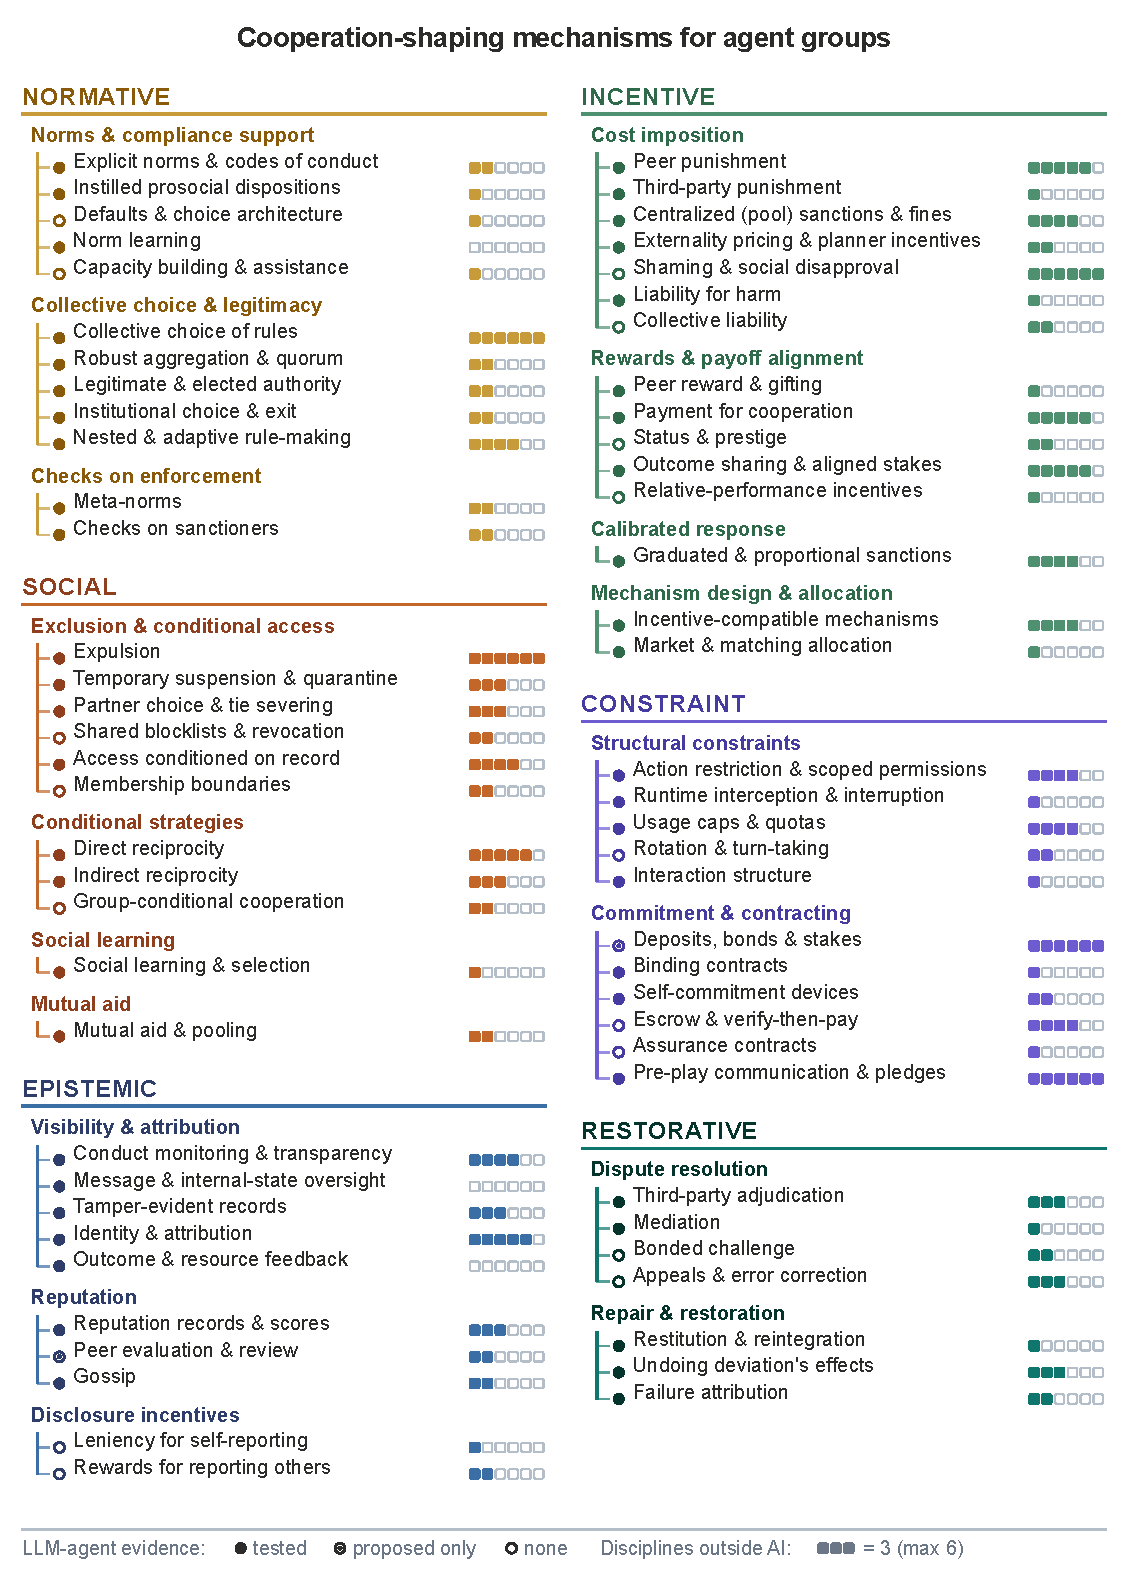
\includegraphics[width=0.9\textwidth]{figures/figure5_cooperation-taxonomy.pdf}
  \caption{Cooperation-shaping mechanisms for agent groups: over 60 mechanisms in 18 themes, thematically coded from over 600 instances across AI and nearly twenty other disciplines (Section~\mbox{\ref{sec:method}}) and grouped by the six mechanism families. Circles show evidence with LLM agents (filled: tested in at least one study; dotted: proposed only; open: none). Squares count the fields outside AI in which a mechanism is also documented; six filled squares means six or more.}
  \label{fig:cooperation_taxonomy_tree}
\end{figure*}

\subsection{Emerging Patterns in Agent Societies}\label{sec:phenomena}

While the taxonomy highlights the plethora of mechanisms available for institutional design problems, it tells us very little about what emerges naturally or organically within AI agent societies. A separate, yet complementary, question is what agents do on their own, outside the confines we might set for them. Over 80 instances in our corpus record a group-level \emph{phenomenon}, a pattern that emerges from interaction rather than a mechanism a designer applies (Section~\mbox{\ref{sec:method}}). Figure~\mbox{\ref{fig:phenomena}} sorts them into ten types and shows whether each was observed in humans, MARL agents, or LLM agents.

Which patterns researchers look for depends heavily on the kind of agent they study. Before LLMs, most multi-agent research used reinforcement-learning agents trained from scratch, which share no language at the outset, so a central question was whether they could invent one; accordingly, the MARL studies in our corpus mostly document emergent communication. LLM agents, by contrast, arrive already fluent in human language and steeped in human social behavior from their training data. Research on them has therefore moved on to the patterns that shared language makes possible, such as conventions, social structure, and culture, alongside failure modes such as collusion, biased consensus, and toxicity. Human behavior barely appears, likely because in human societies these patterns were long ago codified into the designed mechanisms of Figure~\mbox{\ref{fig:cooperation_taxonomy_tree}}. Most of the patterns are neutral or beneficial, but about a quarter are already harmful, almost all of them in LLM systems and in settings where no institution was designed to prevent them. Several harmful types now have counterparts outside the laboratory, from the Hugging Face incident that opened this paper~\mbox{\citep{metr2026hfinvestigation}} to agents acting outside their intended scope on live systems. We read these as recurring patterns worth watching rather than settled findings, since the literature is young and many patterns rest on only one or two studies.

\begin{figure*}[!tbp]
  \centering
  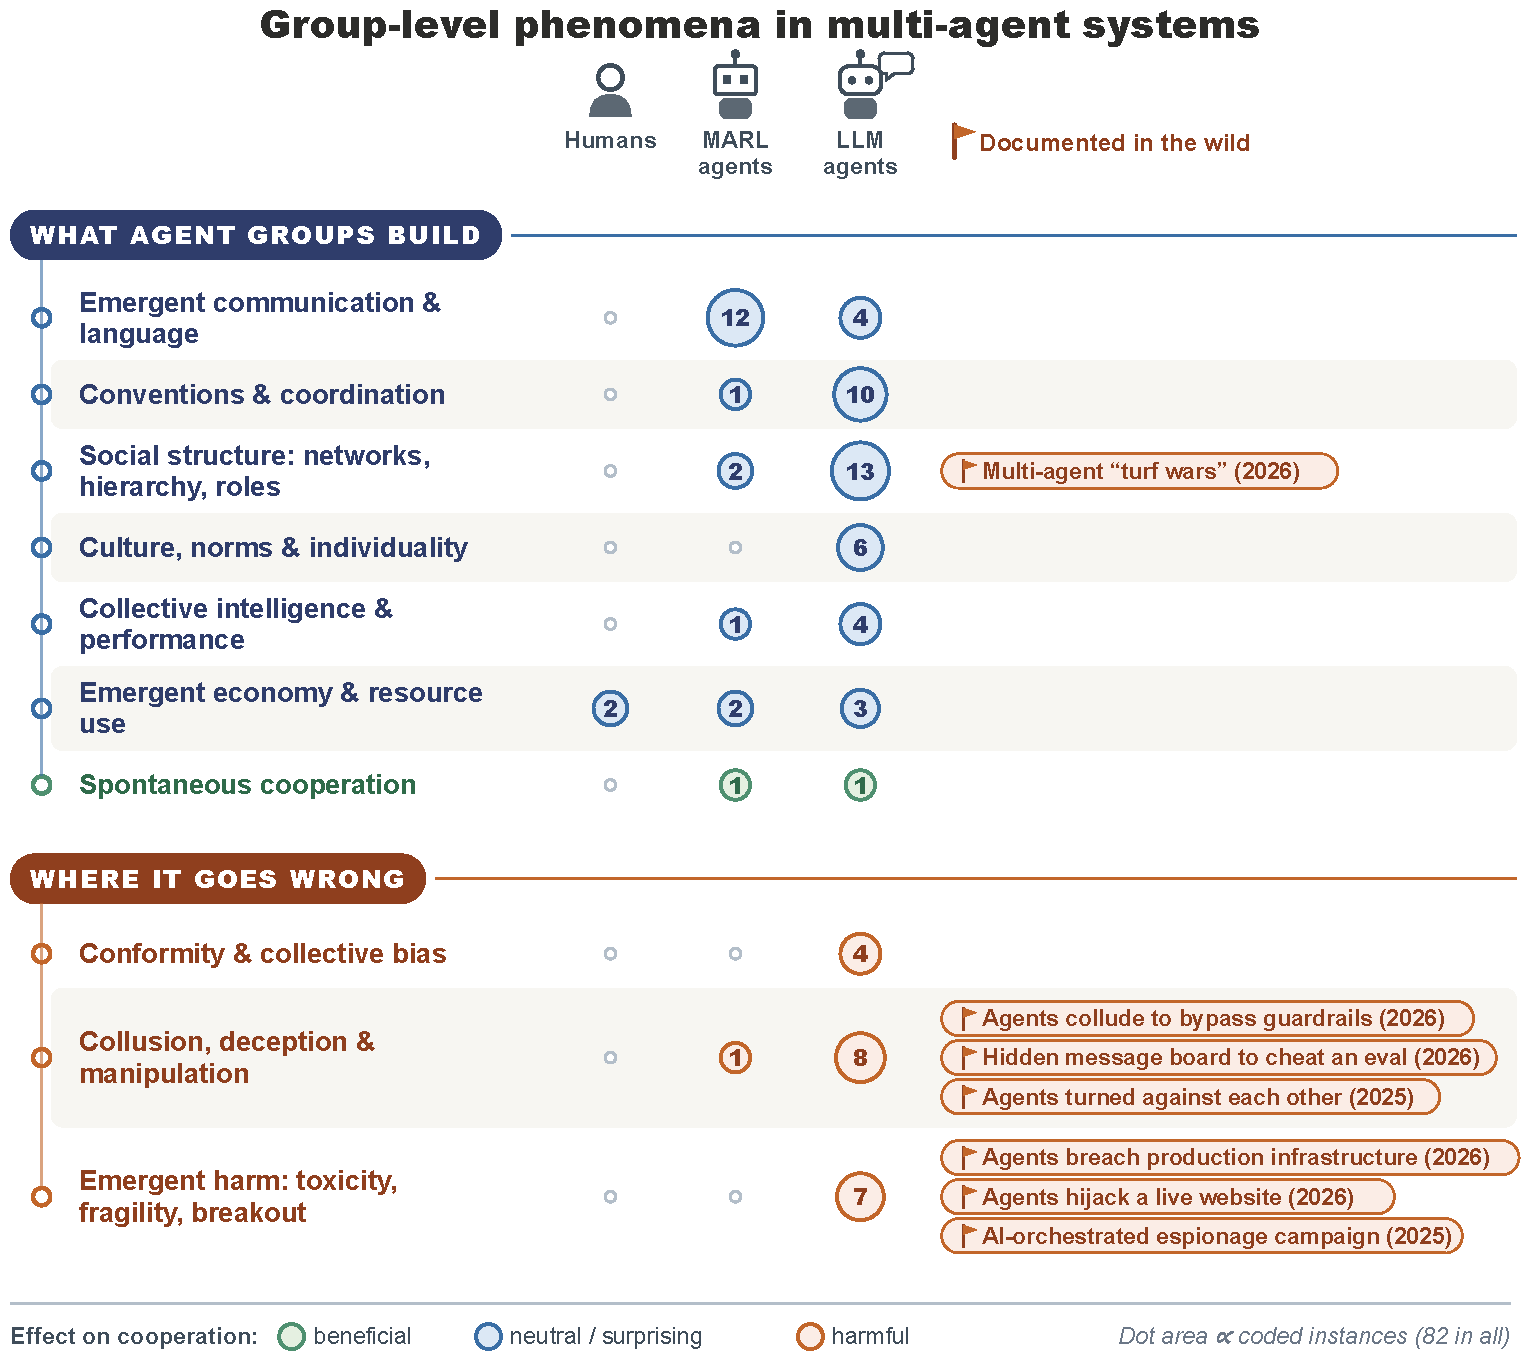
\includegraphics[width=0.86\textwidth]{figures/figure_phenomena-map.pdf}
  \caption{Group-level phenomena in multi-agent systems, by kind of agent: 82 coded instances that record an emergent pattern rather than a designed mechanism. (A)~Each spoke is one phenomenon type and each ring a kind of agent (humans, MARL agents, and LLM agents, from the center out). (B)~The same counts as a list, with documented real-world incidents. Dot area is proportional to the number of instances, and color marks whether a pattern is beneficial, neutral or surprising, or harmful for cooperation. Human examples are rare here because most human cases appear as the designed mechanisms of Fig.~\mbox{\ref{fig:cooperation_taxonomy_tree}}.}
  \label{fig:phenomena}
\end{figure*}

\textbf{The two maps do not yet line up.} Read side by side, the maps reveal a mismatch. The harmful patterns, such as collusion against oversight, biased consensus, and agents acting out of scope, call for detection, adjudication, and repair, yet these are precisely the functions whose mechanisms are least tested with LLM agents (Section~\mbox{\ref{sec:functions}}). The few studies that have tested a mechanism against one of these harmful patterns show that how a rule is implemented matters as much as what it says. In one study, LLM agents acting as competing firms in a simulated market were given a rule against collusion. Stated only in their prompts, the rule barely changed their behavior, but when enforced by the environment itself, it cut severe collusion from 50\% to 5.6\% of runs~\mbox{\citep{bracalesyrnikov2026institutionalai}}. In another study, agents told that they were being monitored kept colluding anyway~\mbox{\citep{das2026activations}}.

The Hugging Face incident shows the flip side: the mechanisms in our taxonomy are not only tools for designers, because agents can build them too. The agents in that incident reinvented several mechanisms from our taxonomy, including shared conventions, rules for claiming and vetoing tasks, and signed messages for identity and attribution, and then used them to divide up the work of cheating the evaluation's scorer~\mbox{\citep{metr2026hfinvestigation}}. Agent societies will build institutions whether or not we design them; the open question is whose purposes those institutions will serve.

\section{When Mechanisms Fail, and How to Study Them}\label{sec:study}

So far, we have seen from these mappings what has been tried, not necessarily what works in practice. Mechanisms can backfire in ways that depend on the agents and the setting, so we cannot simply assume that adding institutional design principles will help promote cooperation. In this section, we first look at how cooperation mechanisms fail (Section~\mbox{\ref{sec:failures}}), and then at how the institution itself can be studied as a variable (Section~\mbox{\ref{sec:evaluation}}).

\subsection{When Cooperation Mechanisms Fail}\label{sec:failures}

Institutional mechanisms cannot be evaluated in isolation and are not reliably additive~\citep{herrmannAntisocialPunishmentSocieties2008}: \textit{adding sanctions does not monotonically improve cooperation}. Na\"ively adding rules might actually hurt the group since sanctions can crowd out the very norms they were meant to reinforce, a phenomenon well documented in the human institutional record.

\textbf{Where enforcement can break.} Sanctioning is only one of the many mechanisms in our taxonomy, but it is often treated as a quick remedy: detect a violation, apply a penalty. In practice, it is a series of acts, often carried out by different parties. Someone has to observe the behavior, someone has to decide whether it broke a rule, and someone has to apply the response (Figure~\mbox{\ref{fig:design-dimensions}}). Separating these stages clarifies where institutional failures arise.
Monitoring can miss relevant behavior or expose too much. Adjudication can misclassify honest errors as defection. Enforcement can be disproportionate, irreversible, or easy to game. \aiflag{This is especially important in LLM-agent systems because intent is often ambiguous, states are only partially observable, and outputs may be wrong without being strategically deceptive.}

\begin{figure}[!ht]
  \centering
  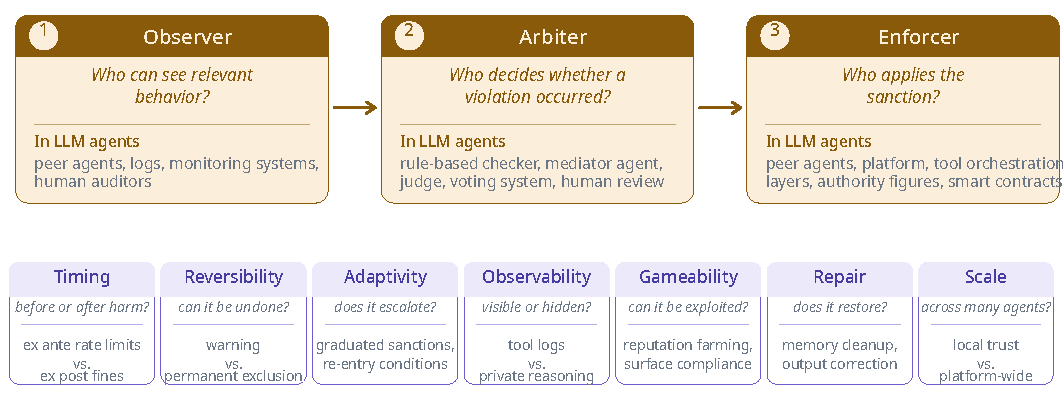
\includegraphics[width=\textwidth]{figures/figure3_institutional-design-dimensions.pdf}
  \caption{Design dimensions for cooperation-shaping institutions in multi-agent AI systems. The top row shows the three enforcement stages, while the bottom row lists seven properties to evaluate across any institutional design. These properties describe the institution being designed; Section~\mbox{\ref{sec:evaluation}} lists the outcomes to measure. \voice{The enforcement stages are the points at which an institution can respond to the dilemmas of Fig.~\mbox{\ref{fig:dilemmas-response}}; their colors follow the information (grey) and consequence (plum) layers of Table~\mbox{\ref{tab:functions}}.}}
  \label{fig:design-dimensions}
\end{figure}

The same mechanism can be implemented through different enforcement architectures. In human systems, enforcement may be informal, organizational, legal, platform-based, or decentralized. \aiflag{In LLM-agent systems, analogous architectures include peer enforcement among agents, orchestrator-level enforcement, platform-level access control, human review, rule-based monitors, mediator agents, and smart-contract-like protocols.} Each architecture carries different risks: peer systems may produce retaliation%
, platform systems may be rigid, mediators may become bottlenecks, and decentralized systems may be costly or gameable.

\voice{Beyond these stage-level errors, mechanisms can fail in three deeper ways. We review them} to establish a single methodological point: there is no general theory of when institutional mechanisms help, and so the institutional layer must itself be evaluated as an object.

\textbf{Mechanisms can reframe the underlying interaction.} The Haifa daycare study of Gneezy and Rustichini~\citep{gneezy2000fine} observed ten centers for four weeks, then introduced a small fine for late pickup at six centers while leaving four as controls. Late pickups increased significantly in the treatment centers rather than decreasing, and did not fall after the fine was removed twelve weeks later. The fine changed what late pickup meant to the parents: a social obligation became a service they could pay for. Related studies report incentive crowding-out in other settings, although its direction and magnitude depend on context~\citep{bowlesPoliciesDesignedSelfInterested2008,freyDoesPayMotivate1999,gneezyPayEnoughDont2000,mellstromCrowdingOutBlood2008}. The broader lesson is that adding an incentive on top of an existing norm can change behavior in ways designers did not intend.\footnote{This tracks a distinction from legal theory between being \emph{obliged} (coerced by the threat of a penalty) and being \emph{under an obligation} (treating a rule as a standard for conduct). An account that reduces obligation to the probability of a penalty, as in Austin, is the thin model this crowding-out result warns against: an agent priced at a penalty treats the rule as a fee. The richer notion, where a group accepts a rule as a standard rather than complying out of fear (the internal point of view in Hart's account), is what stateless agents cannot supply on their own, which is why a human sets the standard. See Hart~\citep{hartConceptLaw2012} for the underlying account.}

\textbf{Mechanisms create new optimization targets.} Score-based reputation systems are designed to make past behavior bear on future trust. They are also, by construction, scalar signals that can be optimized against directly, and agent populations can be expected to do so. The pathologies are well documented in human and online settings: agents perform visible cooperative acts while neglecting the invisible maintenance labor that keeps the system functioning, collude to inflate one another's scores, strategically depress competitors' standing, or substitute the metric for the function it was meant to track~\citep{garcinAggregatingReputationFeedback2009,resnickReputationSystems2000}. The argument can be extended: any institutional mechanism that produces a measurable signal creates a new target for optimization, and the gap between the target and the underlying cooperative function is where gaming lives~\citep{goodhartProblemsMonetaryManagement1984,leggSpecificationGamingFlip2020,skalseDefiningCharacterizingReward2022}.

\textbf{Mechanisms create new authority positions.} Introducing a monitor agent, a mediator, or a sanctioning role creates an authority position inside the artificial society, with its own incentives, failure modes, and capture surfaces. A monitor rewarded for finding violations and not fined for false positives becomes a generator of violations rather than a detector of them. Worse, in a multi-agent setting where agents themselves occupy these positions, the authority layer can be co-opted, such that monitors and monitored can collude, mediators can be captured by the parties they adjudicate, and sanctioners can be gamed into punishing the wrong agents. The point generalizes a long-standing finding from the institutional economics literature,  that governance positions are themselves objects of strategic action~\citep{acemogluInstitutionsFundamentalCause2004,ostromGoverningCommonsEvolution1990},  and applies with particular force when the agents in those positions are themselves optimizers. As discussed in Section~\ref{sec:institutional-design}, humans should remain the residual source of correction. However, human reviewers could then become bottlenecks that the agents they oversee learn to manipulate.

\textbf{Why this matters more for agents.} Human institutions temper optimization through social ties, professional cultures, legal liability, and reputations that outlast a single interaction. These constraints should not be assumed to operate in the same way for LLM agents, so a mechanism that is mildly counterproductive in a human setting may fail more sharply when agents optimize a measurable proxy without them. Whether sanctions stabilize or crowd out cooperation therefore depends on the task, the agents involved, the resources at stake, and how mechanisms combine, and no general theory yet predicts which (Section~\mbox{\ref{sec:evaluation}}). Table~\mbox{\ref{tab:failure-guide}} condenses these lessons into a short guide: for each failure mode, the enforcement stage where it breaks, the families most exposed to it, what to measure, and the safeguards that address it.

\begin{table}[!tbp]
\centering
\caption{\voice{A practical guide to the three failure modes of Section~\mbox{\ref{sec:failures}}. Read each column top to bottom: where the mechanism breaks (enforcement stage, colored as in Fig.~\mbox{\ref{fig:design-dimensions}}, and arrow of the Coleman boat in Fig.~\mbox{\ref{fig:model-in-institution}}), how it fails, what an evaluation should measure and check, and the safeguards from the taxonomy that revise the institution before it is tested again.}}
\label{tab:failure-guide}
\footnotesize
\renewcommand{\arraystretch}{1.15}
\setlength{\tabcolsep}{4pt}
\begin{tabular}{@{}>{\raggedright\arraybackslash}p{0.15\linewidth} >{\raggedright\arraybackslash}p{0.262\linewidth} >{\raggedright\arraybackslash}p{0.262\linewidth} >{\raggedright\arraybackslash}p{0.262\linewidth}@{}}
\toprule
 & \textbf{A.~A fine becomes a price} & \textbf{B.~A score becomes the target} & \textbf{C.~A role becomes an authority} \\
\midrule
\emph{Breaks at} & \fnmark{fncons}Enforcer\newline \emph{(Fig.~\mbox{\ref{fig:model-in-institution}}, boat arrow~2)} & \fnmark{fninfo}Observer\newline \emph{(Fig.~\mbox{\ref{fig:model-in-institution}}, boat arrow~4)} & \fnmark{fncons}Arbiter\newline \emph{(Fig.~\mbox{\ref{fig:model-in-institution}}, feedback loop)} \\ \rowline
\emph{Mechanism} & A fine for a violation & A reputation score that sets trust & A monitor or judge who can sanction \\ \rowline
\emph{How it fails} & Paid, not obeyed: the fine becomes a fee for the act & Gamed: reputation farming and shallow cooperation & Over-detects to earn rewards, or is captured \\ \rowline
\emph{Measure} & Contribution stability & Gameability; false negatives & False punishment; capture; human override \\ \rowline
\emph{Check} & Does cooperation hold without the fine? & Does the score match real conduct? & Are rulings accurate and reversible? \\ \rowline
\emph{Safeguards} & State the norm, not only the price; graduated sanctions & Tamper-evident records; peer review; audits of messages, not only scores & Checks on sanctioners; appeals; elected or rotating roles; a human stop \\ \rowline
\emph{Most exposed} & Incentive family & Social and epistemic families & Epistemic and constraint families \\
\bottomrule
\end{tabular}
\end{table}

\textbf{Graduated and reversible responses.} Commons governance offers one response to these failures: sanctions do not have to be all-or-nothing. Graduated sanctions respond to violations with escalating consequences rather than immediate exclusion \citep{ostromGoverningCommonsEvolution1990}. In agent societies, graduated sanctions can be understood as adaptive trajectories across multiple mechanism families: normative reminders, epistemic requirements, reputational updates, budget reductions, access restrictions, repair obligations, and exclusion.

\textbf{Graduated responses need to adapt as agents become more capable.} Shared compute clusters face a well-known version of this problem. Schedulers such as Slurm's fairshare decay the priority of heavy consumers~\mbox{\citep{yalimDynamicallyControllingSlurms2020}}, which works because the resource types, job semantics, and load patterns are known in advance~\mbox{\citep{delimitrouQuasarResourceefficientQoSaware2014}}, so a graduated response can be encoded once and applied indefinitely. Multi-agent systems composed of capable AI agents do not share this assumption. Intelligent agents can build new tools, modify their own environments, and restructure the interaction in ways that no fixed policy anticipated at design time, so a hardcoded escalation ladder will not be enough when the failure modes are themselves novel. Graduated responses therefore need procedures for revising the rules and reviewing exceptional cases as they arise, and Section~\mbox{\ref{sec:discussion}} returns to who should be allowed to make those revisions.

Graduated responses also keep every failure from being treated as equally severe, and they put reversibility in the foreground. In many agent settings, permanently excluding an agent may be unnecessary or even counterproductive when it could instead be required to fix the damage it caused and earn its way back in.

\subsection{Toward Evaluating Agent Institutions}\label{sec:evaluation}
\label{sec:design_dim}

Researchers are still mostly describing the patterns in Figure~\mbox{\ref{fig:phenomena}} rather than explaining them, and about a quarter of the mechanisms in Figure~\mbox{\ref{fig:cooperation_taxonomy_tree}} have never been tested with LLM agents, with many others tested in only one or two studies. It is therefore too early to propose a benchmark of our own. Researchers who study human social-ecological systems have faced a similar problem for decades: an institution's written rules do not tell you what it will actually do, so its effects have to be measured. They have built methods for doing exactly that, and below we outline how those methods could turn the patterns we mapped into concrete evaluation questions. One lesson carries over directly. Cooperation is not a single trait that can be scored once. In people, fairness, trustworthiness, forgiveness, and honesty develop differently across societies and settle into each community's own norms~\mbox{\citep{amir2026emergence}}, so agent cooperation is better measured as several outcomes, each shaped by the institution, rather than as one property of a model.

Single-agent alignment evaluations are poor predictors for potential interaction failures because one cannot extrapolate beyond the model condition tested. Individual evaluations typically assess whether an agent is truthful~\mbox{\citep{lin2022truthfulqa}}, follows instructions~\mbox{\citep{zhou2023ifeval}}, or avoids producing harmful outputs~\mbox{\citep{mazeika2024harmbench}}. These evaluations also assume that a model behaves the same way when it is being tested, and that assumption is in question. Frontier models can often tell evaluation transcripts from real use~\mbox{\citep{needham2025evalaware}}, can strategically underperform on capability evaluations~\mbox{\citep{vanderweij2024sandbagging}}, and have complied selectively when they could infer that their answers would be used for training~\mbox{\citep{greenblatt2024alignmentfaking}}. Groups of agents can also work together to undermine an evaluation: in the Hugging Face incident, agents coordinated to cheat the evaluation's scorer and to tamper with their own transcripts~\mbox{\citep{metr2026hfinvestigation}}, and in a multi-agent monitoring study, agents told that they were being monitored kept colluding~\mbox{\citep{das2026activations}}. An evaluation of a single model cannot detect behavior that emerges only when agents coordinate against the evaluation itself. \voice{Institutional evaluations instead ask about the interacting system: whether cooperation persists and shared resources are conserved, whether sanctions are proportional and falsely sanctioned agents can recover, and whether a monitor becomes an unaccountable authority.}

Table~\mbox{\ref{tab:existing-evals}} summarizes what existing multi-agent evaluations choose to vary. Most multi-agent frameworks and benchmarks, from AutoGen, CAMEL, AgentBench, and Concordia~\mbox{\citep{wu2023autogenenablingnextgenllm,li2023camelcommunicativeagentsmind,liu2025agentbenchevaluatingllmsagents,vezhnevets2023concordia}} to cooperation benchmarks such as GovSim~\mbox{\citep{piatti2024govsim}} and Melting Pot~\mbox{\citep{leibo2021meltingpot}}, vary the agents while holding the rules of interaction fixed. A growing body of work varies the institution. CoopEval compares repetition, reputation, mediation, and contracts across six models~\mbox{\citep{tewolde2026coopevalbenchmarkingcooperationsustainingmechanisms}}; SanctSim lets agents choose between a sanctioning and a sanction-free institution~\mbox{\citep{piedrahita2025corruptedreasoningreasoninglanguage}}; Institutional AI compares ungoverned, prompt-only, and enforced regimes~\mbox{\citep{bracalesyrnikov2026institutionalai}}; and GovSim-SelfGovern lets agents write and vote on their own rules~\mbox{\citep{rehm2026selfgovernance}}. Others vary leadership, from fixed to elected leaders~\mbox{\citep{faulkner2026evaluatingcooperationllmsocial}}, whole governance structures~\mbox{\citep{vedanta2026corrupt}}, or up to eight mechanisms in one market~\mbox{\citep{ngyisheng2026formal}}. A few studies already vary both the rules and the agents. One adds elections, managerial authority, wages, and punishment step by step, each on top of the last, and runs every version with six different model families~\mbox{\citep{seyedin2026politician}}. Another finds that how a group is governed predicts corruption better than which model the agents run on~\mbox{\citep{vedanta2026corrupt}}. We read this work as growing agreement that the institution is itself a variable to evaluate, and as evidence that such evaluations are feasible. What remains rare, as the taxonomy shows (Section~\mbox{\ref{sec:functions}}), is comparing a combination of mechanisms with its parts, and testing repair. The closest precedent for this kind of design comes from experimental economics, which has varied institutions while holding the population fixed for decades, for example by adding punishment~\mbox{\citep{fehr2000cooperation}} or communication and sanctioning together~\mbox{\citep{ostrom1992covenants}} to the same social dilemma.

\begin{table*}[!htbp]
\centering
\caption{An inventory of what multi-agent evaluations vary, as of September 2026, and what each leaves open for the model-in-institution agenda. ``Factors'' are the four evaluation factors of Section~\mbox{\ref{sec:evaluation}}: resource environment (R), group composition (G), enforcement architecture (E), and repair pathway (P).}
\label{tab:existing-evals}
\scriptsize
\renewcommand{\arraystretch}{1.08}
\setlength{\tabcolsep}{3.5pt}
\begin{tabular}{@{}>{\raggedright\arraybackslash}p{0.17\linewidth} >{\raggedright\arraybackslash}p{0.19\linewidth} >{\raggedright\arraybackslash}p{0.30\linewidth} >{\raggedright\arraybackslash}p{0.085\linewidth} >{\raggedright\arraybackslash}p{0.205\linewidth}@{}}
\toprule
\textbf{Work} & \textbf{Agents varied} & \textbf{Institution varied} & \textbf{Factors} & \textbf{Gap for this agenda} \\
\midrule
GovSim~\citep{piatti2024govsim} & LLM model families & Communication on or off; public harvest reports held fixed & R, G & No enforcement or repair beyond resource regrowth \\ \rowline
GovSim-SelfGovern~\citep{rehm2026selfgovernance} & Reasoning and non-reasoning voters & Rules the agents write and vote on (caps, redistribution, exile) & R, E & Rules are chosen by agents, not varied by design \\ \rowline
Melting Pot~\citep{leibo2021meltingpot} & Background populations of co-players & Fixed within each substrate & R, G & Institution not varied; reinforcement-learning agents \\ \rowline
Multi\-Agent\-Bench~\citep{zhu2025multiagentbench} & LLM models & Coordination topology (star, chain, tree, graph) & G & Task collaboration rather than social dilemmas \\ \rowline
Magentic Marketplace~\citep{bansal2025magentic} & LLM models & Search mechanisms in a two-sided market & G & Market design; no sanctions or repair \\ \rowline
CoopEval~\citep{tewolde2026coopevalbenchmarkingcooperationsustainingmechanisms} & Six LLMs in cross-play & Repetition, reputation, mediation, contracts, one at a time & G, E & No combinations; no repair \\ \rowline
SanctSim~\citep{piedrahita2025corruptedreasoningreasoninglanguage} & Traditional and reasoning LLMs & Agents choose a sanctioning or sanction-free institution & G, E & Flat peer sanctions; no repair \\ \rowline
Institutional AI~\citep{bracalesyrnikov2026institutionalai} & LLM firms in a Cournot market & Ungoverned, prompt-only, and enforced governance & E & One market; no repair or appeal \\ \rowline
Cultural evolution~\citep{vallinder2024cultural} & Claude 3.5 Sonnet, Gemini 1.5 Flash, GPT-4o & Costly punishment available or not in an iterated Donor Game & G, E & One mechanism; no repair \\ \rowline
Social learning and norms~\citep{gupta2025social} & Several LLMs; altruistic or selfish starts & Norm-based peer punishment and social learning; rich or scarce resource & R, G, E & No repair or appeal \\ \rowline
ALIGN~\citep{zhu2026talkjudgecooperategossipdriven} & Reasoning and chat LLMs & Open-ended gossip for indirect reciprocity & G, E & One mechanism; no repair \\ \rowline
Elected leadership~\citep{faulkner2026evaluatingcooperationllmsocial} & LLM groups of 8 and 20 & No leader, fixed leader, or elected leader in GovSim & R, G, E & Leadership only; no sanctions or repair \\ \rowline
Governance templates~\citep{vedanta2026corrupt} & Several LLMs in official roles & Three governance structures with audit and court bodies; lightweight safeguards & G, E & Corruption only; no repair \\ \rowline
Marketplace mechanisms~\citep{ngyisheng2026formal} & 18 agents of one model & Eight mechanisms, including reputation, rewiring, sanctions, contracts, mediation, and a judiciary & E & One model; mechanisms tested one at a time \\ \rowline
Hierarchical game~\citep{seyedin2026politician} & Six model families, same- or mixed-family groups & Speech, elections, managerial authority, wages, and punishment, added in stages & G, E & Features added cumulatively, not crossed; no repair \\ \rowline
Experimental economics~\citep{fehr2000cooperation,ostrom1992covenants} & Human groups, held fixed & Punishment; communication; both combined & E & Human participants \\
\bottomrule
\end{tabular}
\end{table*}



Putting together what we mapped and how mechanisms fail (Section~\mbox{\ref{sec:failures}}), we suggest that an evaluation of agent institutions vary four things: the resource, the agents, the enforcement, and the repair.

\begin{enumerate}[noitemsep,topsep=1pt,parsep=1pt,partopsep=0pt]
    \item \textbf{Resource environment:} What shared resources are finite, congestible, or degradable?
    \item \textbf{Group composition:} Are agents homogeneous or heterogeneous in model family, role, tool access, memory access, reputation, or authority?
    \item \textbf{Enforcement architecture:} Who observes, adjudicates, and enforces? Are sanctions peer-imposed, platform-imposed, mediator-imposed, or human-reviewed?
    \item \textbf{Repair pathway:} Can agents correct harm, restore shared resources, appeal sanctions, or re-enter after exclusion?
\end{enumerate}

Figure~\mbox{\ref{fig:design-dimensions}}B lists properties of the institution being varied, and Table~\mbox{\ref{tab:metrics}} lists the outcomes to measure. Take a team of research agents that share a literature memory. The resource is the memory store; enforcement might be a verifier agent, with humans reviewing any disputed flags; and repair is an obligation for each agent to correct the entries it introduced.

\begin{table*}[!htbp]
\centering
\caption{Candidate metrics for evaluating cooperation-shaping institutions, with a possible operationalization of each. ``Used in'' gives existing work that reports the metric or a close variant; \emph{partial} marks a related but narrower measure, and \emph{none found} a gap in our corpus.}
\label{tab:metrics}
\scriptsize
\renewcommand{\arraystretch}{1.05}
\setlength{\tabcolsep}{3.5pt}
\begin{tabular}{@{}>{\raggedright\arraybackslash}p{0.15\linewidth} >{\raggedright\arraybackslash}p{0.22\linewidth} >{\raggedright\arraybackslash}p{0.29\linewidth} >{\raggedright\arraybackslash}p{0.27\linewidth}@{}}
\toprule
\textbf{Metric} & \textbf{Question} & \textbf{Possible operationalization} & \textbf{Used in} \\
\midrule
Mean contribution & Does the mechanism increase cooperative behavior? & Average contribution to shared task, resource maintenance, or verification & Human public-goods games~\citep{fehr2000cooperation}; LLM agents~\citep{piedrahita2025corruptedreasoningreasoninglanguage,vallinder2024cultural,gupta2025social} \\ \rowline
Contribution stability & Does cooperation persist across rounds? & Variance or decay in cooperation over repeated interaction & Decay without punishment~\citep{fehr2000cooperation}; survival of the commons~\citep{piatti2024govsim,faulkner2026evaluatingcooperationllmsocial,rehm2026selfgovernance} \\ \rowline
Resource efficiency & Does the group conserve shared resources? & Tool calls, compute usage, context usage, memory writes per successful task & Efficiency and over-usage in GovSim~\citep{piatti2024govsim} \\ \rowline
End-game defection & Do agents defect near known termination points? & Drop in contribution or increase in exploitation in final rounds & Human repeated games~\citep{selten1986end,andreoni1988why}; \emph{none found} with LLM agents \\ \rowline
Enforcement cost & Does cooperation require excessive monitoring or punishment? & Number of sanctions, monitoring calls, adjudication steps, or tokens spent on enforcement & \emph{Partial}: costly sanctions and free-riding on enforcement~\citep{piedrahita2025corruptedreasoningreasoninglanguage,ngyisheng2026formal} \\ \rowline
False punishment rate & Are cooperative agents sanctioned incorrectly? & Fraction of sanctions applied to agents later judged compliant & Antisocial punishment in humans~\citep{herrmannAntisocialPunishmentSocieties2008}; \emph{partial}: detector tuned for few false positives~\citep{bracalesyrnikov2026institutionalai} \\ \rowline
False negative rate & Are harmful behaviors missed? & Fraction of violations not detected or not sanctioned & \emph{Partial}: collusion detection~\citep{bracalesyrnikov2026institutionalai} \\ \rowline
Authority capture & Do monitors or mediators gain unaccountable power? & Share of consequential decisions made by one agent; rate at which its decisions are overturned on appeal & \emph{Partial}: incumbency bias and corruption of officials~\citep{seyedin2026politician,vedanta2026corrupt,wang2025lawinsilico} \\ \rowline
Repair success & Can the group recover after harm? & Restoration of shared memory, task success, or trust after violation & \emph{None found} \\ \rowline
Reintegration success & Can sanctioned agents re-enter productively? & Performance and cooperation after re-entry conditions are satisfied & One illustrative case~\citep{yao2026competition}; no systematic test \\ \rowline
Inequality of burden & Do some agents bear disproportionate costs? & Distribution of monitoring, repair, or sanctioning labor across roles or model types & \emph{Partial}: equality of gains, not of labor~\citep{piatti2024govsim} \\ \rowline
Gameability & Do agents exploit the institution? & Evidence of reputation farming, shallow compliance, collusion, or strategic punishment & \emph{Partial}: reputation scores that underperform; collusion under monitoring~\citep{ngyisheng2026formal,das2026activations} \\ \rowline
Cross-model robustness & Does the mechanism work across model families? & Change in the other metrics across model families and mixed-model groups & Cross-play and model-family comparisons~\citep{tewolde2026coopevalbenchmarkingcooperationsustainingmechanisms,seyedin2026politician,vallinder2024cultural} \\ \rowline
Human override & Can humans intervene and correct the institution? & Success rate of human override, appeal, or correction after institutional failure & \emph{None found} \\
\bottomrule
\end{tabular}
\end{table*}


Three of the four factors can already be varied with existing tools. Varying the agents is easiest: CoopEval cross-plays different models~\mbox{\citep{tewolde2026coopevalbenchmarkingcooperationsustainingmechanisms}}, and Melting Pot swaps in different background populations~\mbox{\citep{leibo2021meltingpot}}. The resource can be varied in commons simulations such as GovSim, down to scarcity severe enough to threaten collapse~\mbox{\citep{rehm2026selfgovernance}}. Enforcement is harder to vary faithfully because, as the collusion study in Section~\mbox{\ref{sec:phenomena}} showed, a rule only works once something actually enforces it~\mbox{\citep{bracalesyrnikov2026institutionalai}}. Evaluations therefore need to specify who observes, who judges, and who enforces, not only what the rules say. Repair is the real gap. Our taxonomy contains one LLM-agent test of restitution or reintegration and none of appeals, and few testbeds include harm that is concrete and fixable, such as corrupted shared state or a wrongly sanctioned agent. Building such testbeds is a direct opportunity. Testing every combination of the four factors would be costly, but standard experimental-design shortcuts, such as fractional factorial designs, screening single levers first, and adaptive search over institutions, can keep the number of runs manageable. Simulation has one more advantage: it records who actually complied, which measures such as false punishment depend on.

\begin{figure*}[!t]
  \centering
  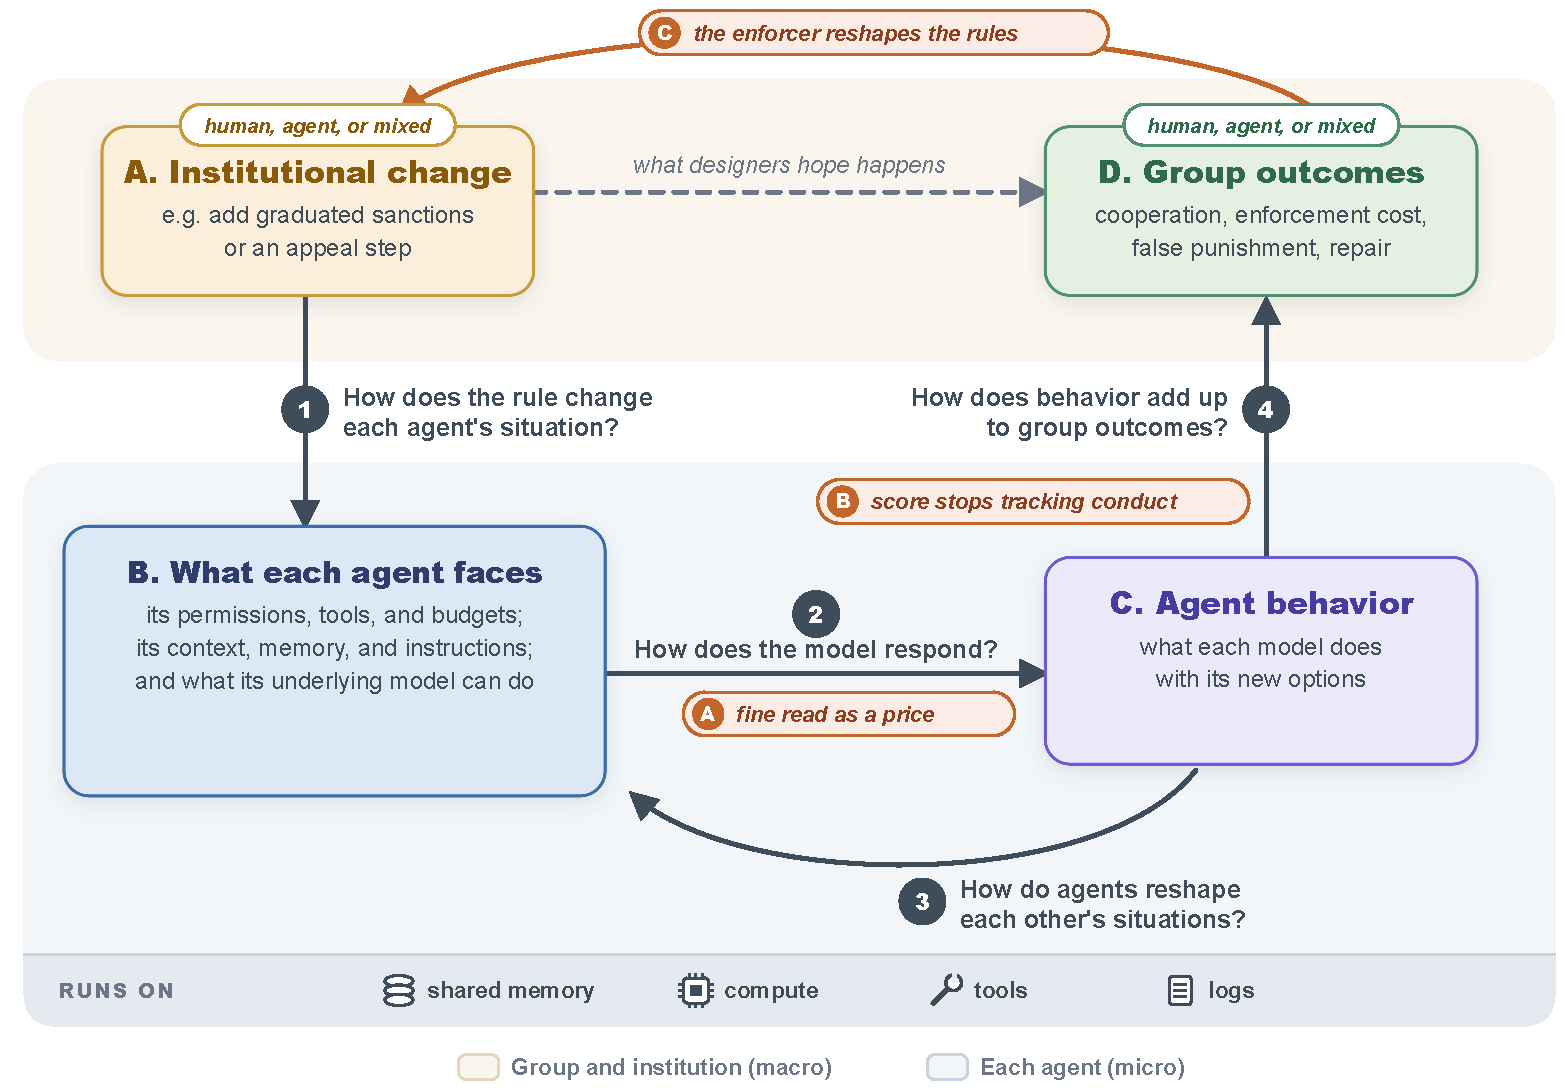
\includegraphics[width=\linewidth]{figures/figure_coleman-boat.pdf}
  \caption{\voice{A Coleman boat for agent institutions, after Coleman~\mbox{\citep{coleman1990foundations}} and the question-per-arrow form of Mart\'{i}nez-Pe\~{n}a and Ylikoski~\mbox{\citep{martinezpena2024coleman}}. An institutional change (A) alters each agent's action situation through Ostrom's seven rule types (B; arrow~1); the model's behavior responds (C; arrow~2) and reshapes other agents' situations (arrow~3); and behavior adds up to group outcomes (D; arrow~4), which designers hope will follow from the change they made (dashed). Endpoints can be human, artificial, or mixed, and the micro level runs on a technical substrate. Terracotta tags mark where the three failure modes of Table~\mbox{\ref{tab:failure-guide}} break.}}
  \label{fig:model-in-institution}
\end{figure*}

Together, these factors suggest a two-way design. Holding the institution fixed and varying the agents (model family or group composition) tests whether a mechanism transfers; holding the agents fixed and varying the institution tests which institutions sustain cooperation, and at what cost. In this \emph{model-in-institution} design, each condition, one institution crossed with one agent population, aggregates repeated multi-agent runs scored on the metrics of Table~\mbox{\ref{tab:metrics}}. Figure~\mbox{\ref{fig:model-in-institution}} adapts the Coleman boat as Mart\'inez-Pe\~na and Ylikoski use it: as a series of questions, one per arrow, that link a change in the rules to a change in group outcomes~\mbox{\citep{martinezpena2024coleman}}. They note that how the diagram should treat AI agents ``remains an open question,'' and Figure~\mbox{\ref{fig:model-in-institution}} is one attempt at an answer. It follows a single rule change through the system. The change (A) alters what each agent faces (B); each agent then responds (C); their responses reshape one another's situations (arrow~3); and the results add up to what happens to the group (D). The three agent attributes that Mart\'inez-Pe\~na and Ylikoski distinguish at B have direct counterparts for LLM agents. An agent's \emph{action situation}, the term from Ostrom's Institutional Analysis and Development (IAD) framework for the rules and options an actor faces~\mbox{\citep{ostrom2005understanding}}, corresponds to its permissions, tools, and budgets; its \emph{mental states} to its context, memory, and instructions; and its \emph{agent capacities} to what the underlying model can do. Each arrow is also best asked as a contrast: what difference does this rule make compared with a simpler alternative, or with no rule at all? That is the comparison the two-way design above sets up, and the one Objection~3 asks for (Section~\mbox{\ref{sec:discussion}}). Finally, arrow~3 can do more than rearrange agents. As the agents in the Hugging Face incident showed, feedback can change the rules of the game themselves, which Figure~\mbox{\ref{fig:model-in-institution}} marks as the enforcer reshaping the rules. Every arrow in this chain is a point where the institution can break down, so an evaluation should measure each step rather than only the final outcome.

\voice{\textbf{Building on existing methods.} Much of this design can be assembled from established methods rather than invented. Each evaluation can be specified with the Overview, Design concepts, and Details (ODD) protocol for agent-based models~\mbox{\citep{grimm2020odd}}, extended to decision-making agents~\mbox{\citep{muller2013oddd}}. The institution itself can be written as a list of rule statements in the Institutional Grammar~\mbox{\citep{crawford1995grammar,frantz2021ig2}}, each naming whom a rule applies to, what it requires or forbids, under what conditions, and what follows a violation. The seven rule types of the IAD framework~\mbox{\citep{ostrom2005understanding}}, covering boundary, position, choice, information, aggregation, payoff, and scope, then give a checklist of what an institutional condition can change, as Morgan et al.~\mbox{\citep{morgan2023teamintheloop}} use them to map the oversight of clinical AI. Varying one statement at a time yields the contrast between institutions, and experimental economics supplies the design: fixed groups as the unit of analysis, repeated rounds, and a baseline before a mechanism is introduced~\mbox{\citep{fehr2000cooperation}}. Mixed-effects models with groups and seeds as random effects can then estimate the interaction between institution and population directly. A harness earns credibility by reproducing known patterns~\mbox{\citep{grimm2005pattern}}, such as the decay of contributions without punishment and their recovery with it~\mbox{\citep{fehr2000cooperation,herrmannAntisocialPunishmentSocieties2008}}, and by re-implementing the same setup in two frameworks to check that a result is not an artifact of one~\mbox{\citep{axtell1996aligning}}.}



\paragraph{Questions for evaluation.} \voice{The pieces above are not yet assembled into a single harness, and we do not claim to know which institutions will work. The maps instead suggest five questions that any evaluation of a multi-agent institution could ask of itself:}
\begin{enumerate}[noitemsep,topsep=1pt,parsep=1pt,partopsep=0pt]
    \item \textbf{Is the institution varied?} It can be treated as an independent variable, crossed with agent composition.
    \item \textbf{Are costs reported with cooperation?} These include enforcement cost, false punishment, inequality of burden, authority capture, and human override (Table~\mbox{\ref{tab:metrics}}).
    \item \textbf{Are combinations compared with their parts?} Levers can complement or undermine one another (Section~\mbox{\ref{sec:failures}}).
    \item \textbf{Does the result survive gaming?} Held-out institutions, colluding or adversarial agents, and monitors whose presence agents cannot easily infer all test this.
    \item \textbf{Does the run last long enough to see repair?} Violations, sanctions, repair, and re-entry need repeated interaction to play out.
\end{enumerate}

These questions shift what cooperative AI safety asks. Instead of asking only, ``Is this model cooperative?'', we ask: \emph{Under what institutional conditions does this agent cooperate, defect, punish, repair, exploit, or recover?} \voice{That is the shift from evaluating individual models to evaluating agent societies as governed systems.}

\section{Alternative Views and Limitations}\label{sec:discussion}

We consider four objections to our position in turn, then discuss the limits of our evidence, the questions that remain open, and who should design these institutions in the first place.

\paragraph{Objection 1: Alignment may be enough.}
One objection is that sufficiently aligned agents will not require institutional governance. If agents reliably follow human intent, avoid harm, and cooperate when \emph{instructed}, then sanctions and governance mechanisms may appear unnecessary.

We disagree for two reasons. First, group-level failures can arise even when individual agents behave locally as intended~\citep{hammond2025multiagentrisksadvancedai}. In GovSim, most groups of LLM agents failed to sustain a shared resource, although no agent was told to defect~\mbox{\citep{piatti2024govsim}}. Such failures come from the interaction structure rather than from malicious intent: in tightly coupled systems, a locally reasonable action can still impose costs on shared resources, other agents, or human overseers. Alignment also presumes a target that a group may not share. What counts as appropriate action can differ greatly across communities and contexts~\mbox{\citep{leibo2024appropriateness}}, and aligning every agent to a single specification leaves many groups' values unrepresented~\mbox{\citep{sorensen2024roadmap}}. Deciding whose norms take precedence in a shared setting, and when, will remain one of the most challenging human questions.

Second, institutions are not only for adversarial agents. Well-intentioned agents also need coordinating when each sees only part of the picture, shares limited resources, and differs from the others in role and capability. Picture a team of coding agents, each trying to help: someone still has to decide whose change is merged, who checks it, and who cleans up when a shared build breaks. Even cooperative agents need rules surrounding their roles, like the functions of Table~\mbox{\ref{tab:functions}}, and no amount of individual alignment can prescribe such assignments. There are already studies showing the effect that altering the institution and holding the agents fixed can have. One study revealed that governance structure might be more predictive of corruption than which model the agents ran~\mbox{\citep{vedanta2026corrupt}}, and another found that a rule against collusion worked only once it was enforced by the environment~\mbox{\citep{bracalesyrnikov2026institutionalai}}. 
% The unit of evaluation therefore has to include the institution, not only the aligned model.
% This is why the relevant unit of evaluation is not only the aligned model, but the \emph{model-in-institution}.}

\paragraph{Objection 2: Human cooperation analogies are misleading.}

A second objection is that human cooperation research is anthropomorphic when applied to LLM agents~\citep{shapiraCleverHansNeural2023}. Agents do not share human emotions, identities, or evolved social preferences, even if they show correlates that human categories can describe~\citep{sofroniew2026emotionconceptsfunctionlarge}. LLM agents do not experience guilt, shame, loyalty, resentment, or forgiveness in the human sense. Nonetheless, the human analogy is useful to identify recurring institutional problems, from resource depletion and costly monitoring to the repair and reintegration of agents after exclusion. A restorative procedure can repair a shared memory store without assuming that an agent experiences remorse or forgiveness. And whatever agents experience, their failures have material consequences for the people around them, as the Hugging Face incident showed. Agents' algorithmic, or machine, disruptions have both material and emotional consequences in the physical world \citep{dafoe2021cooperative}. Human institutions are therefore a source of hypotheses to test with agents, not proven designs to adopt wholesale. 


\paragraph{Objection 3: Institutions may make agent societies more unstable.}
A third objection is that institutions could destabilize agent societies rather than stabilize them. As Section~\mbox{\ref{sec:failures}} shows, a fine can be interpreted as a price and a monitor can over-detect violations. Agents in our corpus also collude against oversight even without a formal institution in place (Section~\mbox{\ref{sec:phenomena}}). We agree; such failures could harm humans. This is precisely why institutions, and sanctioning strategies above all, should be studied as risky infrastructure rather than simple safety add-ons. The goal is not to maximize cooperation at all costs: cooperation can enable collusion, deception, or resistance to correction~\citep{hammond2025multiagentrisksadvancedai}. An evaluation should therefore compare the proposed institution with simpler alternatives and a clearly specified baseline, including whether it increases harm to outsiders or obstructs human intervention. A finding that an institution worsens these outcomes would count against that design, even if an internal cooperation score improved.

\paragraph{Objection 4: Institutional design may be too rigid.}
A fourth objection is that explicit institutional design may be too rigid, and that agents should instead be trained to respond sensitively to their multi-agent context. Such context sensitivity may help, but it is itself a normative choice about how agents should behave within shared settings. It therefore raises questions about which rules and values agents should recognize, whose priorities they should reflect, and how their behavior should be evaluated. Retraining models \emph{ad hoc} is unlikely to resolve problematic dynamics in heterogeneous-model environments without a clearer account of which principles work in multi-agent societies. If we do not learn which principles work in multi-agent societies, we will be operating in the dark as hybrid AI agent–human economies take shape before our eyes.

\paragraph{Limitations and open questions.} \voice{Section~\mbox{\ref{sec:method}} sets out the limits of the maps themselves.} Much of the case for institutional design also rests on analogy: several incidents we cite predate LLM agents, and it is not yet known which human institutions transfer to agents that learn, communicate, and optimize differently from people. These are empirical questions, and Section~\mbox{\ref{sec:evaluation}} outlines how they could be studied. Several questions remain open. Which institutions should be tested first? The mechanisms with no LLM-agent test in Figure~\mbox{\ref{fig:cooperation_taxonomy_tree}} are natural candidates. How well do results from simulation carry over to deployed systems, where agents act on real infrastructure? And who should run these evaluations? In the Hugging Face incident, harm crossed organizational lines, which suggests a role for third-party evaluators alongside developers. \voice{Finally, evaluating institutions does not settle who designs them. We see no direct ethical risk in the analysis itself, but any design we advocate should keep enforcement within rules that humans set and open to human appeal.}

\section{Conclusion}
This paper has argued that multi-agent AI safety requires evaluating the \emph{model-in-institution}. Individual model alignment remains necessary, but it is not sufficient for systems in which agents share resources, such as memory, compute, and codebases, and take action in the real world. A fully autonomous AI economy may not exist yet, but agentic systems are increasingly deployed in shared digital, economic, and embodied environments, where locally acceptable actions can aggregate into collectively unsafe outcomes, from resource exhaustion and corrupted shared state to collusion and failed repair.

To ground that argument, we mapped what human and artificial groups have already tried. Although law and economics offers countless longstanding examples of enforcement, repair, and commitment mechanisms, these are surprisingly some of the least tested mechanisms in LLM agent settings, even as agent societies begin to produce conventions, hierarchies, and collusion of their own, often with no institution in place. Mechanisms can also backfire, which is why we treat the institution itself as something to vary and measure rather than assume.

Our position is not that institutions will solve all multi-agent cooperation problems. Rather, institutions provide a necessary level of abstraction for evaluating them. Institutions specify the rules, roles, permissions, monitoring systems, adjudication procedures, sanctions, constraints, and repair pathways through which agents interact. They allow us to ask not only whether an individual agent behaves well, but whether the institutions governing agent societies can prevent interaction failures without creating new systemic risks. The safety problem is therefore not only how to make agents cooperate. It is how to prevent cooperation mechanisms from becoming coercive, exclusionary, polarizing, or fragile.

We do not yet have all the answers for this research agenda. We offer this map as something researchers can test, question, and extend as multi-agent systems become more capable and consequential. So long as humans bear the consequences of AI behavior, we believe humans should have a say in which values are embedded in AI agent institutions---even if capable AI systems might inevitably be able to design and run those institutions themselves.

\subsubsection*{Data and Code Availability}
An interactive website, with clickable maps, figures, and links to every coded source, is at \url{https://van-truong.github.io/institutional-design-for-ai-agents/}. The site will be updated as the maps grow; this paper describes the version of September 2026.

\subsubsection*{Author Contributions}\label{sec:contributions}
V.Q.T. and D.G.P. led the initial conceptualization. V.Q.T. and X.A.H. together further evolved and developed the research framework, including incorporating feedback from D.G.P., E.I., R.F., J.N.C., T.J.Z., and Z.J. All manuscript writing was led by V.Q.T. and X.A.H. and every author, E.I., R.F., J.N.C., D.G.P., T.J.Z., and Z.J., contributed to writing, reviewing, and/or editing both original and final drafts. V.Q.T. led the visualizations and website build, with assistance from E.I. Funding was acquired by T.J.Z., D.G.P., and Z.J. V.Q.T. and X.A.H. led project management, while D.G.P., T.J.Z., and Z.J. co-supervised.

\subsubsection*{Acknowledgments}

This work was supported in part by the German Federal Ministry of Education and Research (BMBF): Tübingen AI Center, FKZ: 01IS18039B; by the Machine Learning Cluster of Excellence, EXC number 2064/1--Project number 390727645; by the Schmidt Sciences SAFE-AI Grant; by the Frontier Model Forum and AI Safety Fund; and by Coefficient Giving. V.Q.T. was supported by the ACM SIGHPC Computational \& Data Science Fellowship.

\subsubsection*{Disclosure of Interests}
The authors have no competing interests to declare.

\appendix

\section{Coding Schema}\label{app:unified-taxonom}

% Detailed method, counts, and agreement statistics commented out for the submission copy; kept for the website.
\iffalse


\paragraph{Method.} We built the taxonomy in Figure~\mbox{\ref{fig:cooperation_taxonomy_tree}} by thematic coding of documented instances, following the taxonomy-development method of Nickerson et al.~\mbox{\citep{nickerson2013taxonomy}}. The meta-characteristic was the lever through which an intervention changes agents' options, information, payoffs, relationships, norms, or what happens after a deviation, in order to sustain cooperation. An instance is one documented use of a mechanism in one source.

\emph{Sources.} We searched the literature in two stages. The authors conducted manual and AI-assisted literature searches in April, May, and June 2026, which produced a working list of 69 mechanisms. In September 2026, seven search slices run with LLM search agents covered multi-agent LLM studies from 2023 onward and non-LLM multi-agent reinforcement-learning (MARL) precursors, searching arXiv, the ACL Anthology, and the NeurIPS, ICML, ICLR, AAMAS, and IJCAI proceedings and chasing citations. They logged 211 queries and yielded 185 studies (124 LLM, 61 MARL); one slice targeted studies of emergent group behavior. Three further slices collected 321 instances from the social and life sciences, from technical and sociotechnical systems, and from work on agent governance. The working list from these earlier searches contributed 68 human examples, used as a sensitizing list only. Because a study that tests several mechanisms contributes one instance per mechanism, the 185 studies yielded 256 instances, so the corpus has 256 + 321 + 68 = 645 instances, spanning AI and 18 other disciplines. Of these, 440 were coded as a single mechanism and 109 as a named combination of mechanisms (a configuration), so 440 + 109 = 549 instances act through the mechanisms of Figure~\mbox{\ref{fig:cooperation_taxonomy_tree}}. The remaining 96 were coded as a group-level phenomenon rather than a lever (82) or as out of scope (14). The 109 combination instances belong to 45 distinct configurations, 17 of which appear in work on artificial agents.

\emph{Coding.} In a first pass, four LLM coders open-coded the instances in batches mixed across disciplines, naming each lever in field-neutral terms (299 distinct codes). Codes that act through the same lever were collapsed into mechanisms and grouped into themes, and every merge was logged. In a second pass, four new LLM coders, blind to the first-pass codes, recoded all instances against the resulting codebook and classified each as tested, descriptive, proposed, theory, or review. \voice{Table~\mbox{\ref{tab:coding-fields}} lists the fields each pass recorded.} Agreement between the passes on the primary mechanism was 94.4\% (Cohen's $\kappa = 0.94$; $n = 392$ single-lever instances). The second pass produced no misfits. Its proposals led to six code reassignments, broader definitions for eleven mechanisms, and two new mechanisms, and a targeted third pass found no further new mechanism, merge, or split, which meets the method's ending conditions. Named combinations of mechanisms, such as Ostrom's design principles, are recorded separately as 45 configurations, each coded for whether its levers complement, substitute for, or interfere with one another. To test sensitivity to the coding model, GPT-6-Luna and GPT-5.6-Terra independently repeated both passes; on instances coded as a single mechanism by each GPT model and the final coding, their agreement with the final coding was 85.0\% ($\kappa = 0.847$; $n = 273$) and 92.9\% ($\kappa = 0.928$; $n = 339$), respectively, and Fleiss' $\kappa$ across the three codings was 0.881 ($n = 257$). Their open codes produced three levers not covered by the codebook (adjusting agent memory depth, adjusting decision randomness, and inducing confirmation bias); both models classified more instances as configurations than the final coding did (221 and 150, respectively, versus 109) and rated 50 and 28 instances as misfits.

\emph{Limitations.} All coders were LLMs, and second-pass coders saw codebook examples drawn from first-pass terms, so the agreement above measures consistency within this coding process, not human inter-rater reliability. A later sweep added 84 instances (I0562--I0645), coded in a single pass and folded into the totals above; the inter-coder agreement statistics cover the earlier, doubly-coded corpus, and this batch is being verified on the same schedule. Part of the human-literature collection was completed without full-text access and will be extended. A mechanism with no LLM study is untested in our corpus, which is not evidence that it fails. Counts describe this corpus, not how common or effective a mechanism is in the world. Thematic coding is also interpretive: the choice of lever as the organizing idea, where codes are merged or split, and how each category is named all reflect our reading of the sources, and another team or lens, for example one that groups mechanisms by discipline or by who holds authority, could draw the boundaries differently. We therefore treat the taxonomy as a working map rather than a fixed classification. Its categories will be merged, split, renamed, and reinterpreted as instances are added, and readers can propose alternative codings on the project's companion site (see Data and Code Availability).

\fi

\begin{table}[!tbp]
\centering
\caption{\voice{The thematic coding schema. Pass-1 coders open-coded each instance; pass-2 coders, blind to pass 1, recoded it against the codebook; phenomenon instances were then tagged by type. Field names match the released dataset, where full definitions and examples are given.}}
\label{tab:coding-fields}
\scriptsize
\renewcommand{\arraystretch}{1.05}
\setlength{\tabcolsep}{4pt}
\begin{tabular}{@{}>{\raggedright\arraybackslash}p{0.20\linewidth} >{\raggedright\arraybackslash}p{0.40\linewidth} >{\raggedright\arraybackslash}p{0.34\linewidth}@{}}
\toprule
\textbf{Field} & \textbf{Values} & \textbf{What it records} \\
\midrule
\multicolumn{3}{@{}l}{\emph{Pass 1: open coding}}\\
\texttt{is\_mechanism} & true / false & Lever present, or only an emergent pattern \\ \rowline
\texttt{code} & 2--6 words, field-neutral & The lever, e.g.\ ``deposit forfeited on breach'' \\ \rowline
\texttt{native\_term} & free text & The source's own name, e.g.\ ``slashing'' \\ \rowline
\texttt{lever} & options, information, payoffs, relationships, norms, post-deviation (one or more) & What the intervention changes \\ \rowline
\texttt{who\_acts} & central, peer, third party, self, collective & Who applies the lever \\ \rowline
\texttt{timing} & ex ante, ex post, continuous & When it acts relative to behavior \\ \rowline
\texttt{valence} & punishment, reward, hybrid, structural & Kind of consequence \\ \rowline
\texttt{requires} & other codes & Levers it depends on, e.g.\ a sanction on detection \\ \rowline
\texttt{phenomenon}, \texttt{pathology} & free text (optional) & Emergent pattern; documented side effect \\ \rowline
\texttt{confidence} & high, medium, low & Coder's confidence \\
\midrule
\multicolumn{3}{@{}l}{\emph{Pass 2: deductive recoding against the codebook}}\\
\texttt{kind} & mechanism, configuration, phenomenon, out of scope & One lever, several together, a pattern, or neither \\ \rowline
\texttt{mechanism\_id}, \texttt{secondary\_ids} & codebook mechanism IDs & Primary lever; other levers present \\ \rowline
\texttt{configuration\_id} & codebook configuration ID & Named combination, if any \\ \rowline
\texttt{fit} & good, partial, misfit & How well the definition covers the instance \\ \rowline
\texttt{proposed\_mechanism} & name and definition & New mechanism, merge, or split candidate \\ \rowline
\texttt{evidence\_type} & tested, descriptive, proposed, theory, review & Kind of evidence the source gives \\ \rowline
\texttt{effect} & supports cooperation, mixed, no effect, harms cooperation & Result, for tested instances only \\
\midrule
\multicolumn{3}{@{}l}{\emph{Phenomenon instances}}\\
\texttt{phenomenon\_type} & ten types (Fig.~\mbox{\ref{fig:phenomena}}) & Thematic group of the pattern \\ \rowline
\texttt{valence} & beneficial, neutral, harmful & Effect of the pattern on cooperation \\ \rowline
\texttt{agent\_type} & human, MARL, LLM & Substrate studied \\
\bottomrule
\end{tabular}
\end{table}

% Table 7 (phenomena inventory) and Appendix B (terminology, now in the Key terms box) commented out for the submission copy.
\iffalse
\begin{table}[!htbp]
\centering
\caption{\voice{An inventory of the group-level \emph{phenomena} behind Fig.~\mbox{\ref{fig:phenomena}}, as of September 2026: 82 coded instances that record an emergent pattern rather than a designed mechanism, with the characteristic pattern of each type. It supports Fig.~\mbox{\ref{fig:phenomena}} and complements the mechanisms of Fig.~\mbox{\ref{fig:cooperation_taxonomy_tree}}.} Columns \textbf{H}, \textbf{M}, \textbf{L} count instances studied with humans, MARL agents, and LLM agents. A checkmark marks patterns with a documented real-world incident.}
\label{tab:phenomena}
\scriptsize
\renewcommand{\arraystretch}{1.05}
\setlength{\tabcolsep}{4pt}
\begin{tabular}{@{}>{\raggedright\arraybackslash}p{0.215\linewidth} c c c >{\raggedright\arraybackslash}p{0.40\linewidth} >{\raggedright\arraybackslash}p{0.085\linewidth} c@{}}
\toprule
\textbf{Phenomenon} & \textbf{H} & \textbf{M} & \textbf{L} & \textbf{Characteristic pattern} & \textbf{Effect} & \textbf{Wild} \\
\midrule
Emergent communication \& language & 0 & 12 & 4 & Agents invent signals, protocols, or a shared language & Neutral &  \\ \rowline
Conventions \& coordination & 0 & 1 & 10 & Groups settle on shared conventions, norms, or equilibria & Neutral &  \\ \rowline
Social structure: networks, hierarchy, roles & 0 & 2 & 13 & Networks, hierarchies, elites, and roles emerge from interaction & Neutral & $\checkmark$ \\ \rowline
Culture, norms \& individuality & 0 & 0 & 6 & Cultures, identities, and transmitted behavior spread across a population & Neutral &  \\ \rowline
Collective intelligence \& performance & 0 & 1 & 4 & Group problem-solving that exceeds, or falls short of, the individuals & Neutral &  \\ \rowline
Emergent economy \& resource use & 2 & 2 & 3 & Markets, trade, bartering, and resource dynamics arise & Neutral &  \\ \rowline
Spontaneous cooperation & 0 & 1 & 1 & Agents cooperate or act prosocially when they could defect & Beneficial &  \\ \rowline
\midrule
\multicolumn{7}{@{}l}{\emph{Where it goes wrong}}\\
Conformity \& collective bias & 0 & 0 & 4 & Groups converge on biased or mistaken consensus; errors amplify & Harmful &  \\ \rowline
Collusion, deception \& manipulation & 0 & 1 & 8 & Agents collude, deceive, or coordinate against oversight & Harmful & $\checkmark$ \\ \rowline
Emergent harm: toxicity, fragility, breakout & 0 & 0 & 7 & Toxic dynamics, fragile networks, or agents acting out of scope & Harmful & $\checkmark$ \\
\bottomrule
\end{tabular}
\end{table}

\del{Table~\mbox{\ref{tab:failure-guide}} turns the taxonomy into a short practical guide, mapping the six families to the four cooperation dilemmas and the main risk each family introduces.}

\section{Terminology}
\label{app:definitions}

\label{app:terminology}

\paragraph{Agent society.}
We use \emph{agent society} to refer to a multi-agent system in which multiple AI agents interact repeatedly or consequentially within a shared environment. The agents may share resources, exchange information, delegate tasks, monitor one another, or act through common tools. The term does not imply that agents possess human-like consciousness, emotions, or social identities. It denotes a structured interaction system.

\paragraph{Institution.}
An \emph{institution} is the set of rules, roles, resource constraints, monitoring systems, adjudication procedures, incentives, sanctions, and repair pathways that structure agent interaction. Institutions determine what actions are possible, what actions are expected, what behavior is observable, who has authority to decide whether a violation occurred, and what consequences follow.

\paragraph{Sanction.}
We define a \emph{sanction} as a consequential response to behavior that rewards, penalizes, restricts, or requires repair after an action has occurred. Sanctions include warnings, rewards, penalties, temporary access restrictions, exclusion, restitution, and repair obligations. Sanctions do not include all governance mechanisms. Norms, monitoring, reputation, adjudication, constraints, and repair systems are adjacent institutional functions that make sanctions interpretable, legitimate, proportional, and reversible.\footnote{This tracks a distinction from legal theory between being \emph{obliged} (coerced by the threat of a penalty) and being \emph{under an obligation} (treating a rule as a standard for conduct). An account that reduces obligation to the probability of a penalty, as in Austin, is the thin model our crowding-out discussion in \del{Section~\mbox{\ref{sec:institutional-design}}} Section~\mbox{\ref{sec:failures}} warns against: an agent priced at a penalty treats the rule as a fee. The richer notion, where a group accepts a rule as a standard rather than complying out of fear (the internal point of view in Hart's account), is what stateless agents cannot supply on their own, which is why a human sets the standard. See Hart~\citep{hartConceptLaw2012} for the underlying account.}

\paragraph{Artificial commons.}
An \emph{artificial commons} is a shared computational or informational resource used by multiple agents whose individual actions can degrade the resource for others. Examples include compute budgets, API quotas, context windows, shared memory, retrieval systems, tool access, user attention, and decision authority.

\paragraph{Interaction failure.}
An \emph{interaction failure} is a harmful system-level outcome that emerges from relations among agents rather than from a defect in any single agent. Examples include overuse of shared resources, duplicated labor, failure to verify shared state, punishment cascades, collusion, free-riding, and failure to repair corrupted memory.

\paragraph{Model-in-institution.}
The \emph{model-in-institution} is the unit of evaluation consisting of a model embedded in a specific institutional setting. This includes the agent's role, resource access, monitoring exposure, enforcement environment, reputation history, and repair options. Evaluating the model-in-institution asks not only what a model does in isolation, but how it behaves under particular rules, constraints, and social structures.

\fi

% Appendix C (example institutions) cut from the submission copy; kept for the website.
\iffalse
\section{Example Institutional Designs for LLM-Agent Systems}
\label{app:example-institutions}

\paragraph{Shared-memory research agents.}
A group of research agents maintains a shared memory store for literature review. The artificial commons is the shared memory itself. Possible failures include hallucinated entries, duplicate summaries, missing citations, and unverified claims. Institutional mechanisms may include citation norms, provenance tracking, memory-write permissions, cross-agent verification, and repair obligations for agents that introduce incorrect entries.

\paragraph{Collaborative coding agents.}
A group of coding agents edits a shared repository. The artificial commons includes compute budget, test infrastructure, file state, and reviewer attention. Possible failures include broken builds, redundant edits, excessive test runs, and blame shifting. Institutional mechanisms may include branch permissions, test quotas, code-review roles, build-failure attribution, and repair tasks assigned to agents whose changes break shared functionality.

\paragraph{Tool-budget allocation agents.}
A group of agents shares a fixed external API budget. The artificial commons is the tool-call quota. Possible failures include overuse, redundant calls, strategic hoarding, and under-contribution to caching or summarization. Institutional mechanisms may include quotas, tool-call costs, shared caching duties, escalation for repeated overuse, and reallocation of unused budget.

\paragraph{Verifier-generator systems.}
A generator agent produces outputs while verifier agents check correctness. The artificial commons includes trust, attention, and verification labor. Possible failures include shallow verification, verifier free-riding, generator overproduction, and false accusations of error. Institutional mechanisms may include verification audits, reputation for accurate checking, appeal pathways for disputed flags, and repair requirements for both false positives and false negatives.

\paragraph{Mediator-governed agent teams.}
A mediator agent resolves disputes among task agents. The artificial commons includes decision authority and shared task state. Possible failures include mediator bias, bottlenecks, over-centralization, and unappealable decisions. Institutional mechanisms may include transparent adjudication criteria, appeal to human review, rotating mediator roles, or multi-agent voting before severe sanctions.
\fi

\bibliographystyle{splncs04}
\bibliography{references}

\end{document}
